\documentclass[subeqn]{article}

\title{The Twin Instrument\footnote{We are grateful to Paul Devereux, James 
Fenske, Cheti Nicoletti, Carol Propper, Atheen Venkataramani, Marcos 
Vera-Hernandez and Frank Windmeijer, along with seminar audiences and discussants 
at CMPO Bristol, ESPE, NEUDC, CSAE, The University of Essex, The University of 
Oxford, the Barcelona GSE summer forum and the RES conference for helpful 
comments.  We thank Emilia Del Bono, Climent Quintana-Domeque, Pedro R\'odenas, 
Libertad Gonz\'alez, Anna Aevarsdottir, Martin Foureaux Koppensteiner and Ryan 
Palmer who have very kindly shared data and/or source code from their work.}}
\author{Sonia Bhalotra\thanks{The University of Essex.
Contact: srbhal@essex.ac.uk} 
\and Damian Clarke\thanks{The University of Oxford. 
Contact: damian.clarke@economics.ox.ac.uk}}
\date{\today}


%*******************************************************************************
\usepackage{amsmath}
\usepackage{amssymb}
\usepackage{appendix}
\usepackage{blindtext}
\usepackage{bm}
\usepackage{booktabs}
\usepackage{breqn}
\usepackage{caption}
\usepackage{color} \pagecolor{white}
\usepackage{dcolumn}
\usepackage{epsfig}
\usepackage{epstopdf}
\usepackage[capposition=top]{floatrow}
\usepackage{lastpage}
\usepackage{longtable}
\usepackage{lscape}
\usepackage{multirow}
\usepackage{natbib} \bibliographystyle{abbrvnat}\bibpunct{(}{)}{;}{a}{,}{,}
\usepackage{pdfpages}
\usepackage{rotating}
\usepackage{setspace}
\usepackage{subcaption}
\usepackage{url}
\usepackage{wrapfig}


%*******************************************************************************
\setlength\topmargin{-0.375in}
\setlength\textheight{8.8in}
\setlength\textwidth{5.8in}
\setlength\oddsidemargin{0.4in}
\setlength\evensidemargin{-0.5in}
\setlength\parindent{0.25in}
\setlength\parskip{0.25in}

\newcommand{\twinfolder}{"/home/damiancclarke/investigacion/Activa/Twins"}
\DeclareMathOperator{\plim}{plim}

%*******************************************************************************
\begin{document}
\begin{spacing}{1.4}

\maketitle
\begin{abstract}
 The incidence of twins has been used to identify the impact of changes in 
 fertility on measures of investment in children born prior to the twins, and
 the emerging consensus in this literature is that there is no evidence of a
 quantity-quality trade-off. We argue that the standard approach is flawed.
 Even if twin conception is random, bringing twins to term is a function of
 maternal health which is difficult to fully observe and which tends to be
 correlated with child quality, rendering the instrument invalid. The neglect
 of this fact in the existing literature will tend to lead to under-estimation of 
 the quantity-quality (Q-Q) trade-off and so could contribute to explaining the 
 negative results in the literature. Our contention that women who produce twin 
 births are positively selected is demonstrated using data from richer and poorer
 countries. Using large samples of microdata from developing countries and from 
 the USA which include indicators of maternal characteristics including health, 
 we show that a significant trade-off emerges upon correcting for these biases. 
 We show that this result is likely to be only a \emph{lower} bound of the true
 Q-Q trade-off and discuss how to estimate the size of these bounds.
\\
\end{abstract}
\hspace{4mm}\textbf{\small JEL codes}: J12,J13,C13,D13,I12. \\

\newpage
%*******************************************************************************
\section{Introduction}                             \label{TWINscn:intro}

Talk about Q-Q
Talk about twins
Talk about early life and fetal origins --$>$ links to health, but not twinning.

%*******************************************************************************
\section{Twins}                                    \label{TWINscn:literature}
The ocurrence of twins has fascinated people, not least of all social 
scientists, for as long as recorded history exists. Stories of Romulus and 
Remus, the mythological founders of Rome, date from at least the fourth century 
BC. However, the first use of twins as an exogenous increase in family size in 
the economic literature came much later, in \citet{RosenzweigWolpin1980}.

\citet{RosenzweigWolpin1980} proposed to incorporate twins into an estimation
strategy in order to circumnavigate problems of the joint determination of child 
quantity and quality first raised by \citet{Becker1960,BeckerLewis1973,
BeckerTomes1976}.  Under a number of assumptions, they show that twins as an 
increase to family size will be sufficient to directly identify the interaction
between quality and quantity.  As well as the occurrence of twins pushing at
least some families above their desired total fertility, this requires that 
twin births are random.  Empirically then, \citet{RosenzweigWolpin1980} estimate 
the Q--Q trade-off, accounting for the increase in rates of twinning by parity 
(a biological relationship)\footnote{Such a relationship is an empirical 
regularity in all data examined. \citet{RosenzweigWolpin1980} report rates which 
increase by parity in USA.  In DHS data a similar pattern is observed, as 
presented in figure \ref{TWINfig:bord}.}, and by total number of births (a 
mechanical relationship).  Beyond these variables, twinning must be random to
produce consistent estimates.\footnote{It is important to note that in their
original paper this \emph{is} tested formally.  The authors report that a joint
test of the effect of farm size, non-farm earnings and parental education on the
rate of twins per births did \emph{not} allow for the rejection of no 
statistical effect.}

The twin instrument has been widely used since.  As well as its use in the 
estimation of the quantity-quality trade-off (\citet{RosenzweigWolpin1980, 
Blacketal2005, Angristetal2010, Caceres2006}, among others), it has been used to
estimate the effect of childbearing on female labour force participation 
\citep{RosenzweigWolpin1980b,Jacobsenetal1999,AngristEvans1998}, and the effect 
of unwed childbearing on marriage market outcomes, poverty and welfare receipt 
\citep{BronarsGrogger1994}.  Typically, estimation is based on two-stage least
squares, with the set of controls included in the first- and second-stage 
varying slightly over time.

Table \ref{TWINtab:Lit} documents the principal studies in the Q--Q trade-off 
literature where twins are employed.  Along with the data sample and time period 
under study, we list the set of controls included in each case.  The more recent
wave of these studies make a similar conditional randomness assumption, however
refurbish the controls in IV estimate to include variables such as a mother's 
race and her educational attainment.  In some cases the validity of such 
assumptions is probed by regressing twinning on observable family outcomes, or 
testing for the equality of means of certain characteristics between twin and
non-twin families. \citet{Blacketal2005}, \citet{Lietal2008} and 
\citet{Sanhueza2009} report joint F-tests suggesting that twinning is not related 
to parental education in their data samples, while \citet{RosenzweigZhang2009} 
report t-tests showing equality of means across twin and non-twin groups. 
However, as is well known and acknowledged in each case, any such tests are at 
best partial evidence in support of instrumental validity. While twins can be 
shown to be unrelated to observable or measured characteristics, similar tests 
cannot be run for variables which are either unobservable, or not recorded in 
survey data. We return to this point in the following sections.



Make point about medical literature.\\
Make point about IVF\\
Make point about R,Z type invalidity


%*******************************************************************************
\section{Data and Estimation Samples}              \label{TWINscn:data}
\subsection{Data}                                  \label{TWINsscn:data}
\subsection{Estimation Samples}                    \label{TWINsscn:samples}
\subsection{Descriptive Statistics}                \label{TWINsscn:descriptives}



%*******************************************************************************
\section{Methodology}                              \label{TWINscn:method}
Empirical analyses of the quality-quantity trade-off focus on producing 
consistent estimates of $\beta_1$ in the following equation:
\begin{equation}
\label{TWINeqn:RF}
educ_{ij}=\beta_0+\beta_1 fert_{j} + \bm{X}\bm{\beta}+u_{ij}.
\end{equation}
Here, quality is proxied by the educational attainment of child $i$ in family 
$j$, ($educ$) and fertility ($fert$) is measured as the total births in a child's
family.  A vector of family and child controls is included, denoted $\bm{X}$.  As
has been extensively discussed in prior literature, estimation of $\beta_1$ using
OLS with cross-sectional data will result in biased coefficients given that child 
quality and quantity are jointly determined \citep{BeckerLewis1973,
BeckerTomes1976}, and given that unobservable parental behaviours and attributes 
influence both fertility decisions, and investments in children's education 
\citep{Qian2009}.

\subsection{Quantity-Quality with Twins}           \label{TWINsscn:methodQQ}
One proposed solution has been to employ 2SLS estimation, where fertility is 
is instrumented using twin births.\footnote{Other instruments and methodologies 
are also used including gender mix of children \citep{Angristetal2010}, policy 
experiments \citep{Qian2009}, and historical time series variation in schooling 
\citep{BleakleyLange2009}}  The corresponding first stage is:
\begin{equation}
\label{TWINeqn:firststage}
fert_{j}=\pi_0+\pi_1 twins_{j}+\bm{X}\bm{\pi}+\nu_{j},
\end{equation}
where $twins_j$ is an indicator for whether the $n^{th}$ birth in a family is a 
twin birth. As described in section \ref{TWINsscn:samples}, the sample in each 
case is the so-called $n+$ group, consisting of children born before birth $n$ 
in families with at least $n$ births.  As such the twins themselves are excluded 
from the estimation sample.\footnote{Typically, the argument is made that twins 
are different to single births, and hence should not be compared in analysis.}
The logic, in quasi-experimental terms, is that existing children (the subjects) 
are randomly assigned either one (control group) or two (treatment group) 
siblings.

Consistent estimation of $\beta_1$ can thus proceed provided (among other
things) that instrumental validity holds:
\begin{equation}
\label{TWINeqn:IVvalid}
\plim_{N\to \infty} \frac{1}{N}\sum_{i=1}^N twin_ju_{ij}=0
\end{equation}
The typical challenge in IV estimates arises when considering 
(\ref{TWINeqn:IVvalid}); as the error term $u_{ij}$ consists, by nature, of 
unobservable components, whether or not the equality holds cannot be tested 
formally.  There is however nothing which stops us from partially testing 
(\ref{TWINeqn:IVvalid}) by removing a subset of observable components from $u_{ij}$
and testing whether their covariance with $twin_j$ is significantly different
from zero.  The error term $u$ in (\ref{TWINeqn:RF}) is a function of a large 
number of elements:
\begin{equation}
\label{TWINeqn:IVbias}
\begin{split}
u=f(\text{maternal health stocks, fertility behaviour, positive pregnancy investments,}  \\
\text{parental education, fetal environment,}\ldots)
\end{split}
\end{equation}
While many of the relevant elements are either completely or partially 
unobservable, some of these variables, such as maternal education and partial 
measures of health stocks and behavious, can be observed.  Thus a partial test 
of the twin methodology consists of estimating the following regression.
\begin{equation}
\label{TWINeqn:twinreg}
twin_{j}=\alpha_0 + \bm{X}\bm{\alpha}_1 + \bm{S}\bm{\alpha}_2
                  + \bm{H}\bm{\alpha}_3 + \varepsilon_{j}.
\end{equation}
Here $\bm{X}$ refers to the initial vector of family and child controls, $\bm{S}$
to additional family socioeconomic variables such as income and parental 
education, and $\bm{H}$ to maternal health variables.  

If twin birth is indeed an event which is as good as random, the coefficients
on maternal health and family socieoeconomic variables in the above regression
should not be significantly different to zero.  We thus test the following 
hypothesis:
\begin{equation}
\label{TWINeqn:twintest}
H_0: \bm{\alpha}_2 = \bm{\alpha}_3 = 0.
\end{equation}
Rejection of the null would raise difficulties in proceeding with IV estimation 
using the twin instrument. Of course, if the rejection of the null were only due 
to one or a number of \emph{observable} element(s) which predicted twinning, 
these variables could simply be included in the first and second stages above, 
much like occurs with maternal age and race in the existing literature.  However, 
more generally it would be difficult to be argue for instrumental validity if 
twinning is shown to depend upon (a limited set of) measurable family 
characteristic or choice variables, while many similar variables are not observed.

Given the biological demands placed on a mother pregnant with twins, we may 
expect that healthier mothers, or mothers with more resources to invest in their
pregnancy are more likely to take twin conceptions to term.  Similarly, we may
suspect that mothers more able to invest in their children during pregnancy will 
also be more able to invest in their child's human capital after birth.  If this 
is the case, we would see that (at the very least) $\bm{\alpha_2}>0$.  

An alternative test of whether twins appear to be as good as random consists of 
comparing women who give birth to twins with those who give birth to singletons 
\emph{before} these children are born.  If twin births are as good as random, 
the two groups of mothers should appear identical before these births occur.
In order to compare health stocks before twins, we run tests comparing the rate
of infant mortality---a completely predetermined variable---of children in each 
of the $n+$ groups described above.  If, as we contend, healthier mothers are 
more likely to give birth to twins, this should be captured in lower infant 
mortality rates (IMR) in early births.

Assuming additive separability of the elements in the omitted error term, we can 
re-write $u_{ij}$ from (\ref{TWINeqn:firststage}) and (\ref{TWINeqn:IVbias}) as:
\[ u_{ij}=u^S_{ij}+u^H_{ij}+u^*_{ij}. \]
Here $u^S_{ij}$ and $u^H_{ij}$ correspond to the (observable) elements included 
as $\bm{S}$ and $\bm{H}$ in (\ref{TWINeqn:twinreg}), while $u^*_{ij}$ represents 
the remaining (unobserved) components.  We can thus re-write our IV estimate for 
$\beta_1$ as:
\begin{equation}
\label{TWINeqn:betabias}
\hat\beta_1^{IV} = \beta_1 + 
\plim_{N\to \infty} \frac{1}{N}\sum_{i=1}^N twin_j(u^S_{ij}+u^H_{ij}+u^*_{ij})
\end{equation}
Typically, this is the coefficient estimated in the existing twin literature 
which assumes that twinning is a conditionally exogenous event.  If, however, the 
likelihood of taking twin conceptions to term increases for healthier and/or 
wealthier mothers, we should include $\bm{S}$ and $\bm{H}$ in the first and 
second stages, giving
\begin{equation}
\label{TWINeqn:betacloser}
\hat\beta_1^{IV,S+H} = \beta_1 +
\plim_{N\to \infty} \frac{1}{N}\sum_{i=1}^N twin_ju^*_{ij},
\end{equation}
where the superscript $S+H$ signifies that socioeconomic and health variables 
have been included as additional controls.  What's more, if both the likelihood
that a woman takes twins to term and a family's subsequent investment in child 
human capital are positively correlated with positive health behaviours and other 
positive socioeconomic variables such as parental education, we would expect that:
\begin{equation}
\label{TWINeqn:moves}
\hat\beta_1^{IV}>\hat\beta_1^{IV,H}>\hat\beta_1^{IV,S+H}>\beta_1.
\end{equation}
It should be noted in the above series of inequalities that even conditional upon
socioeconomic and health variables, IV estimation will \emph{not} result in a
consistent estimate of $\beta_1$ if twinning is correlated with unobservable
elements in $u^*_{ij}$.  We return to this point, and how to bound $\beta_1$ in
the following sub-section.

NOTE: Angrist Pischke first stage F-statistics when more than one endogenous
regressor.

%*******************************************************************************
\subsection{Bounding the Q-Q Trade-off}            \label{TWINsscn:methodBounds}
In the previous subsection, Q-Q estimation using twins is motivated in equations 
(\ref{TWINeqn:RF}) and (\ref{TWINeqn:firststage}).  Consistent IV estimation 
imposes the (strong) prior belief that twin births can be excluded from the 
second stage equation, or that the sign of $\gamma$ in the following is equal to 
zero:
\begin{equation}
\label{TWINeqn:Conley}
educ_{ij}=\beta_1 fert_j + \gamma twin_j + \bm{X}\bm{\beta} + u_{ij}.
\end{equation}
As we discuss above, this will not be the case if maternal health controls 
omitted from (\ref{TWINeqn:RF}) are correlated with both the likelihood of taking
twin conceptions to term, and with eventual measures of child quality.

However, even in cases such as this where we are not confident that $\gamma=0$,
we can still estimate bounds on the Q-Q tradeoff if we are confident in making
some statement of prior belief about the distribution from which $\gamma$ is 
drawn.  \citet{Conleyetal2012} describe such a process, which they refer to as 
\emph{plausible exogeneity}.  We invoke this terminology here, and refer to 
twins as a plausibly exogenous event, implying that we have reason to believe 
that $\gamma$ may be close to, but not necessarily precisely equal to, zero.
Specifically, we are concerned that healthier mothers are more likely to give
birth to twins, and, all else constant, healthier mothers are more likely to be 
able to invest more in children post-pregnancy.  Thus, $\gamma$, the coefficient 
on twins, reflects the interaction between the partial correlation of a mother's 
health and her likelihood of giving birth to twins, and the partial correlation 
between her health and child quality.

In this paper we estimate $\beta_1$ under a range of assumptions regarding the
true nature of $\gamma$.  Firstly we estimate $\beta_1$ by simply assuming a
support assumption for $\gamma$: namely that $\gamma$ falls between zero (implying 
instrumental validity) and some (positive) number $\delta$:
\begin{equation}
\label{TWINeqn:uci}
\gamma \in [0,\delta].
\end{equation}
This is a relatively weak assumption, however, as \citet{Conleyetal2012} show,
it allows for us to recover a `union of confidence intervals' (hereafter UCI) 
for estimates of $\beta_1$ over the entire support of $\gamma$.  This UCI, then, 
provides bounds for $\beta_1$ even in the case that twin exogeneity does not 
strictly hold. We also estimate by imposing a stronger prior: specifically we 
fully specify the distribution of $\gamma$ as:
\begin{equation}
\label{TWINeqn:ltz}
\gamma \sim U(0,\delta).
\end{equation}
This stronger assumption allows for a tighter estimate of the bounds on 
$\beta_1$.  \citet{Conleyetal2012} provide a full derivation of this result, and 
we follow them in referring to this as a local-to-zero (LTZ) approximation.

Assumptions (\ref{TWINeqn:uci}) and (\ref{TWINeqn:ltz}) depend upon the values
of $\delta$ which we believe hold in the case of twinning and the Q-Q equation.
As such, we estimate both specifications over a wide range of values for 
$\delta$,  
%*******************************************************************************


\section{Results}                                  \label{TWINscn:results}
\subsection{Twinning}                              \label{TWINsscn:twinning}
In table \ref{TWINtab:TwinDHS} we regress a child's twin status (one if a twin, 
zero if a singleton) on their mother's health, education, and a range of other 
demographic and family characteristics.\footnote{In our principal specification, 
the full set of controls are country, child year of birth, and age dummies; a 
cubic function of mother's age at time of birth; mother's age at time of first 
birth; mother's education and education squared; and mother's height and BMI. 
We cluster standard errors at the level of the mother.}  These results suggest
that twin births are not random, even after conditioning on maternal age and 
child birth order as is typical in the recent twin literature summarised in table
\ref{TWINtab:Lit}. The inclusion of a full set of country and year-of-birth
dummies (not displayed in table \ref{TWINtab:TwinDHS}) will capture any 
systematic trend in the frequency of twin births across time or regions, and 
country dummies will absorb all time invariant differences in the probability 
of a twin birth across countries. The estimated coefficients and signs support 
the idea discussed in section 4 that higher investments (for example in maternal 
health) required to maintain multiple healthy fetuses in utero may result in 
non-random twin births. We return to the mechanism by which twin selection may
occur in the following section.

Initially, results from the pooled DHS data are presented as this provides a 
particularly large sample with which to test the hypothesis of twin exogeneity. 
This is presented in table \ref{TWINtab:TwinDHS} column (1) and provides 
considerable evidence that live twin births are related to family choice 
variables such as education (tests for the joint significance of socioeconomic 
variables and health variables are rejected with p-values of $<$0.00).  
Regressions displayed here are estimated by OLS, however are robust to 
alternative functional forms and estimation methods.\footnote{Significant and 
quantitatively similar results are found if a logit model is estimated rather 
than a linear probability model, and when running separate models for twinning at 
each birth order. Similarly, if we run the regression at the level of the mother 
or include any combination of fertility measures, similar patterns are observed.
Alternatively, rather than running a regression we can run (unconditional) balance 
of characteristics tests by twin status.  These are available in the online 
appendix (table \ref{TWINtab:Balance}).  The findings are similar.}

Columns (2)--(5) suggest that these results, especially when considering 
maternal health, are not the result of only the most low income countries, or
only the post-IVF time period.  Given that the frequency of multiple births 
increases in cases where the mother undergoes fertility treatment, column (5) 
presents regression results for births in a period not potentially 
affected by IVF.\footnote{In order to be conservative, we estimate for the period 
preceeding 1990, the date which coincides with the first reported successful 
use of IVF in South Africa, an early-adopter among DHS countries.}  Pre- and 
post-1990 results are qualitatively similar although education is no longer 
significant prior to 1990 (in the smaller sample). Mother's height and BMI:
measures of health stocks, are positively correlated with twinning regardless
of the sample.  Similarly, this result is not driven by a particular country
or region.  Figure \ref{TWINfig:arrows} provides evidence that healthy women (as 
proxied by height) are significantly more likely to have twins in nearly all of 
the 68 countries included in DHS surveys.  Along with higher average rates of 
twinning in countries with taller women, a positive within-country gradient 
exists, with taller women in a given country more likely to have twins than their 
shorter counterparts. The size of DHS estimates are considerable. Increasing a
woman's height by 1 standard deviation increases the probability of twinning by 
0.44\% (as compared to a mean rate of twins of 1.85\%).

Results for the infant mortality test described in the previous section are
presented in table \ref{TWINtab:IMR}.  In row 1, we regress IMR for first-borns
on the twin status of second-borns.\footnote{IMR is defined as 1 for children
who die before their first birthday.  We remove from the sample any children who
were not yet 1 at the time of the following birth, as these children have not
yet been entirely exposed to the risk of infant mortality.}  Mothers who have 
second-born twins have much lower rates of infant mortality \emph{before} the 
twins than women who had second-born singletons.  This suggests that mothers of 
twins are healthier when considering pre-determined measures of health.  
Similarly, the rates of infant mortality among first- and second-borns are much 
lower in families of women who have third-born twins than in those who have 
third-born singletons.  This holds for all parity levels examined.

Much of the existing twin literature focuses on the USA, or other developed
countries. In table \ref{TWINtab:TwinNHIS}, we provide similar regressions for 
women in the USA based on the full set of NHIS surveys.  These results show
that twins are not as good as random, even in the context of a country with 
a more developed healthcare system and social safety nets. Taller mothers,
heavier mothers, and mothers who don't smoke prior to conception (a positive
health behaviour) are significantly more likely to have twins.

The dependence of twinning on positive maternal health stocks and behaviours is
a consistent and quantitatively important phenomenon in all data sets we have
examined.  We have compiled data and run similar regressions using vital 
statistics data from the USA, Brazil, Spain, Scotland and Sweden, and 
additional survey data from Chile and the United Kingdom (see tables 
\ref{TWINtab:TwinNVSS}--\ref{TWINtab:SwedenTwin} for results).  In each case,
the probability of twinning increases as mothers become more healthy and are
less likely to engage in risky health behaviours before and during pregnancy.
Along with the results described in tables \ref{TWINtab:TwinDHS} and 
\ref{TWINtab:TwinNHIS}, these additional sources of data show that mothers
who consume alcohol, tobacco or other drugs, who suffer from chronic disease 
or who have less access to prenatal care are significantly less likely to twin.

Finally, if twinning is related to positive health stocks and behaviours of
prospective mothers and families, we can examine how rates of twinning respond
to time-series variations in (female) health outcomes.  While only suggestive,
as many other environmental variables may explain changes in twinning, 
time-series evidence from the USA leads to similar conclusions.  Figure
\ref{TWINfig:USTwin} plots the rate of twinning from vital statistics data since
birth type (single or multiple) was first recorded.  Interestingly, the rate of
twins has increased steadily over time, even before the advent of IVF and other
fertilisation treatments.  This is in line with increasing trends in female
health over this period, which is proxied by female life expectancy and plotted
in the same figure.


%*******************************************************************************
\subsection{Selection into twinning: mechanisms}   \label{TWINsscn:selection}
In a wide variety of contexts, healthier women are more likely to give birth to
twins.  There are a number of competing hypotheses which may explain why this is
the case.  Firstly, it may simply be the case that healthier mothers are more 
likely to conceive twins.  This may reflect some underlying biological process, 
such as that mediated by follicle stimulating hormone as discussed in 
\citet{Hall2003}.  Secondly, conditional on conceiving twins, healthier mothers 
may be more likely to take both fetuses to term.  Finally, it may be the case 
that (conditional on conceiving twins and taking them to term), healthier mothers 
may be more likely to survive the birth, and hence appear in survey or vital 
statistics data.  In broad terms we will refer to these as the conception 
mechanism, the gestation mechanism and the birth (survival) mechanism.

When considering IV estimates with twins, any of these processes is sufficient 
to invalidate causal inference insofar as observing twins depends upon hard 
to measure maternal behaviours and characteristics.  Nonetheless, we may be 
interested in determing which of these are the relevant channels in explaining 
the results from the previous section.  Particularly, the mechanism may be 
relevant when considering the use of the instrument.  For example, if twins are 
less likely \emph{only} due to selective maternal death, then as mothers become 
more likely to survive childbirth (ie moving from high maternal mortality 
countries to low maternal mortality countries), threats to instrumental validity 
become less relevant.

We test these mechanisms below.  In order to determine whether twin selection
could be entirely explained by selective maternal survival, we follow 
\citet{Aldermanetal2011} in simulating estimates under the counterfactual 
scenario that unhealthy women---who are more likely to die in childbirth---%
were all carrying twins. Using DHS data described in section 
\ref{TWINsscn:data}, we observe a woman's height, BMI, pregnancy outcomes, and 
the maternal mortality status of all her sisters.  As we do not observe health 
stocks of women who died in childbirth, we assume that her sister's health 
(height and BMI) is a reasonable proxy for the health of the woman who died 
within 42 days of giving birth (which is classed as a maternal death).  Appendix 
figure \ref{TWINfig:survival} shows that maternal mortality is much higher among 
more unhealthy women.  Women shorter than the mean height of 155.5 cm are 
considerably more likely to suffer maternal death, with this being particularly 
so below heights of 145cm.

To test the potential importance of maternal survival in explaining twin 
selection, we simulate observations for the number of women who, according to 
DHS data, would exist in the sample if it were not for the fact that they died 
in childbirth.  We then examine the coefficients of interest in our twin 
regression (\ref{TWINeqn:twinreg}), if all unhealthy women who died were 
pregnant with twins, while all healthy women who died were not.  As this relies 
on a binary `healthy vs unhealthy' distinction, we define this in various ways, 
based on height and BMI.  These results are presented in table 
\ref{TWINtab:Alderman}.  The first column shows the estimated coefficients on 
height and BMI in the unaltered sample of women from DHS countries where 
maternal mortality data is available.  In this sample, a BMI increase of 1 
point is associated with a 0.046\% increase in the probability of twinning. The 
remaining columns add in observations based on maternal mortality rates among 
sisters of surveyed women.  For example, in the second column, we examine the 
effect of adding to the sample unhealthy and healthy women based on the maternal 
mortality rate in each group, and then assuming that all unhealthy women would 
give birth to twins, and all healthy mothers would not. As expected, this 
reduces the importance of positive maternal health in predicting twinning, with 
the coefficient on BMI falling from 0.0460 to 0.0437. The other columns continue 
in this manner, however using continually less conservative assumptions in 
assigning members to the unhealthy group who are defined as giving birth to 
twins. Even in the final column, where the entire bottom half of the 
anthropometric distribution is assumed as being unhealthy, the coefficient on 
both height and BMI remains positive and significant.\footnote{Examining 
selection in this way (as per \citet{Aldermanetal2011}) is only one way to 
examine the effect of selection on estimated coefficients.  An alternative 
measure as proposed by \citet{Lee2009} involves trimming the control and 
treatment group (in our case unhealthy and healthy mothers), to account for 
differential selection by treatment status.  This results in bounds estimates 
of the effect of treatment (good health) on the outcome variable (twinning). We 
report Lee bounds in appendix table \ref{TWINtab:Lee}, however note that these 
bounds are based on the assumption that treatment is random, which here it is 
not.  Nonetheless, \citet{Lee2009} bounds agree with the simulated estimates in 
table \ref{TWINtab:Alderman}, providing further evidence that selective maternal 
survival is not enough to explain the correlation between maternal health and 
twinning.}

These results suggest that selective maternal death is not enough to explain
why healthier mothers are more likely to have twins. Turning to the gestation 
mechanism, we are able to test whether less healthy women who are pregnant with 
twins are more likely to miscarry than healthier women who are also pregnant 
with twins.  In one DHS survey (Nepal), data on miscarriages as well as the 
type of miscarriage (single or multiple fetuses), is recorded.  We thus run a 
series of regressions where miscarriage is the dependent variable, and the 
independent variables are a measures of poor maternal health, whether the 
pregnancy is single or multiple, and interactions between pregnancy type and 
poor maternal health.  We would expect that both poor maternal health and a 
non-singleton pregnancy increase the likelihood of miscarriage, however we are 
interested in determing if more unhealthy mothers are \emph{more} likely to 
miscarry twins than healthy mothers carrying twins.  Thus, we are interested in 
testing if the coefficients on the interaction terms are significantly larger 
than zero.

These regression results are reported in table \ref{TWINtab:Miscarry}.  As 
expected, columns (1) and (2) suggest that more unhealthy and less educated
women are more likely to report ever miscarrying.\footnote{These results hold 
conditional and unconditional on total fertility.}  Maternal health stocks are 
proxied by height and BMI, where (negative) outcomes for these variables such as 
underweight and very underweight are based on ICD-10 definitions. Turning to the 
interaction terms, although standard errors are reasonably large due to the low 
frequency of twinning, women who are unhealthy (as proxied by a very low BMI), 
and with no education are significantly more likely to miscarry with twins.  
Using a richer set of variables from administrative data in the USA and Spain, 
similar regressions are run.  The results in appendix tables 
\ref{TWINtab:USAMiscarry} and \ref{TWINtab:SpainMiscarry} suggest that, 
depending on the context, less educated women and women who report consuming 
alcohol during pregnancy are more likely to miscarry twins than mothers with 
higher education and who do not consume alcohol.

%*******************************************************************************
\subsection{The twin instrument and the Q-Q trade-off} \label{TWINsscn:QQtwins}
Results from section \ref{TWINsscn:twinning} show that twinning is not as good
as random, even when conditioning on race, maternal age, and even parental 
education. Healthier mothers are more likely to have twins. If these mothers 
also invest more after birth, the Q-Q trade-off will be under-estimated (we can 
see this by considering the term $twin_ju^H_{ij}$ in equation 
(\ref{TWINeqn:betabias}).  However, progressively including additional health
controls in our first and second stage equations should drive IV estimates in 
the direction of the true Q-Q trade-off from below.

Conversely, OLS estimates are typically thought to over-estimate the true 
magnitude of the Q-Q trade-off.  If unobserved parental behaviours favour both
lower fertility and higher child human capital,\footnote{As a (highly stylised) 
example, consider a prospective mother's eventual labour market plans. A mother 
who plans to join the labour market may prefer fewer children, facilitating more 
immediate labour force participation, but have more resources to invest in child
quality.} OLS estimates of $\beta_1$ will be negatively biased, and hence 
\emph{more} negative than the true trade-off.  As items are removed from the
error term and included in the principal equation to be estimated by OLS, we thus 
expect that these estimates should approach the true parameter from above.

We examine this intuition by estimating $\beta_1$ from (\ref{TWINeqn:RF}) by OLS 
and IV. Our principal data is the large DHS sample, where quality is measured by
school Z-score, a child's educational attainment compared to his or her country
birth cohort.  After considering DHS estimates we turn to NHIS data from USA.

Table \ref{TWINtab:OLS} reports pooled OLS estimates from all DHS data, and in 
low and middle-income country groups. OLS is estimated separately by the 2+, 3+,
and 4+ fertility groups, and included in appendix table \ref{TWINtab:OLSplus}.

\subsubsection{The twin instrument: estimates of the Q--Q trade-off}
In table \ref{TWINtab:IVAll}, we turn to IV estimates using twins.  As we outline 
in section \ref{TWINsscn:methodQQ}, the assumption of `as good as random' twin 
births is unlikely to hold, even when conditioning on the augmented set of 
controls proposed in (\ref{TWINeqn:twinreg}). If this is the case, we will also 
be unable to consistently estimate $\beta_1$ using twin births.

However, it is likely that the $\beta_1$ which we estimate using twin births 
will provide us with a strict lower bound of the magnitude of the Q-Q trade-off 
as outlined in (\ref{TWINeqn:betacloser}). We expect that the bias in this 
estimate is due to those mothers who invest more in their children in utero, or 
who have greater initial health endowments, being more likely to give birth to 
twins resulting in larger family sizes. At the same time, we expect healthier 
mothers to invest more in their children after birth resulting in higher 
quality children. By relegating health variables to the error term, these two 
positive correlations will result in a positive bias on the fertility 
coefficient estimated via IV. In order to determine the effect that these 
omitted variables have on estimates of the Q-Q trade-off, we turn to results for 
equation (\ref{TWINeqn:RF}), both first omitting, and the including, maternal 
health and socioeconomic variables.

The main specification is displayed in the top row of table \ref{TWINtab:IVAll}, 
with separate columns for the 2+, 3+ and 4+ sample groups. For each parity 
group, the base case (controlling for maternal and child age, country, and year 
of birth) results in insignificant, and at times weakly positive, estimates of 
the effect of an additional birth on a child's educational attainment. These 
results suggest that the inclusion of maternal health and socioeconomic controls 
may be of considerable importance. Despite the lack of results when using
the `typical' set of twin controls from the twin Q--Q literature, including 
health (columns 2, 4 and 6) reduces point estimates on fertility from an effect 
of approximately 0\% of a standard deviation, to -3 or -4\% of a standard 
deviation in standardised educational attainment. Further, conditioning on 
maternal education results in slightly more precise estimates, suggesting a 
statistically significant (or close to statistically significant in the case
of the 2+ sample) Q--Q trade-off of at least 3 or 4\%.

In low- and middle-income country data, the inclusion of health indicators in 
the twin instrument does have an important effect on IV estimates, moving as
hypothesised in (\ref{TWINeqn:moves}).  In table \ref{TWINtab:NHISAll}, we 
present identical estimates based upon NHIS data from the USA.  As this survey
focuses on health, as well as standardised educational attainment, we examine
the effect of additional siblings on the reported health of children.

%*******************************************************************************
\subsubsection{Heterogeneity}
Theoretical derivations of the Q--Q model are based on the assumption that all
children in a family are of the same quality. More recent work (for example the 
theoretical work of \citet{AizerCunha2012}) has loosened this assumption. Among 
other things, this allows for reinforcing behaviours by parents in child human 
capital investment decisions.\footnote{An empirical review of early life human 
capital and reinforcing versus compensating behaviour, (however not explicitly 
related to the Q--Q hypothesis), is provided by \citet{AlmondMazumder2013}.} If 
this is the case, the coefficient $\beta_1$ may vary by children in the family. 
More generally, $\beta_1$ may be context specific, depending upon the returns to 
human capital in a given time-period or economy.

Empirically, we find that estimates of the Q-Q trade-off are heterogeneous 
across birth orders, country income level, and gender of the child affected by 
the additional birth.  The magnitude and significance of the results is lowest 
when considering the effect on the first-born child of moving from two to three 
births (the 2+ group), and higher when considering moving from three to four 
births or four to five births. However, in lower fertility environments the 
effect is, as expected, concentrated on lower birth orders. The third row of 
table \ref{TWINtab:IVAll} suggests that in middle-income countries the effect is 
largest on first borns, and progressively smaller, but still considerable, at 
higher birth orders.

Estimates of the magnitude of the Q--Q trade-off by country income level suggest 
that the trade-off is considerably larger in middle rather than low-income 
countries. In low-income countries point estimates on fertility suggest 
(insignificant) trade-offs centred around 2-3\% of a standard deviation, while in 
middle-income countries results are significant, and considerably larger,
reaching as much as 9\% of a standard deviation: only slightly lower than OLS 
estimates for this group.

Similarly, effects of the Q-Q trade-off are considerably different depending upon 
a child's gender. In appendix table \ref{TWINtab:gend} we present regression 
results estimated separately by the gender of the index child. These results 
suggest that females may bear the brunt of additional births, with estimates
being negative and significant for girls, while insignificant for male children. 
Interestingly, recent empirical of the Q--Q trade-off from other (middle income)
contexts finds similar gender-biased results \citep{SouzaPonczek2012}.

%NOTE that in April 2012 draft, there was some different results discussed here
%that are no longer included.


%*******************************************************************************
\subsection{Bounding the Q-Q trade-off}            \label{TWINsscn:resultBounds}
The results from the previous subsection provide consistent estimates of 
$\beta_1$ via 2SLS \emph{if} the full set of controls completely account for 
those characteristics and behaviours which predict giving live birth to twins. 
However, given that we have shown that twinning is predicted by a wide range of 
health behaviours, and given that maternal health variables in these datasets 
do not exhaustively capture all aspects of health stocks and behaviours, it 
seems unlikely that all relevant variables are included in these specifications. 
As such, we turn to \citeauthor{Conleyetal2012}'s \citeyear{Conleyetal2012} 
methodology to estimate bounds for the Q-Q trade-off.  

As outlined in section \ref{TWINsscn:methodBounds}, this involves the definition 
of some prior belief over the sign and magnitude that the coefficient on 
twinning would take in the structural equation \ref{TWINeqn:Conley}. Results 
are displayed in figures \ref{TWINfig:ltz2} and \ref{TWINfig:ltz3}, and in 
table \ref{TWINtab:Conley}. At each point on the horizontal axis of figures 
\ref{TWINfig:ltz2} and \ref{TWINfig:ltz3}, the bounds for $\beta_1$ are 
displayed, along with the corresponding point estimate under the assumption 
that $\gamma$ is distributed $\sim U(0,\delta)$. Dashed lines present the 95\% 
confidence interval, while the solid line represents the point estimate.


%*******************************************************************************
\section{Conclusion}                               \label{TWINscn:conclusion}
Twin births are not random.  Indeed, they appear to be far from it, in a wide
variety of environments, time periods and contexts.  Based on a considerable 
body of evidence compiled from vital statistics and survey data from low- and 
high-income countries, we demonstrate that mothers with greater health stocks 
and those who engage in positive health-related behaviours are much more likely 
to take twins to term.  

\newpage
\section*{Figures}
\begin{figure}[htpb!]
\centering
\begin{subfigure}{.5\textwidth}
  \centering
  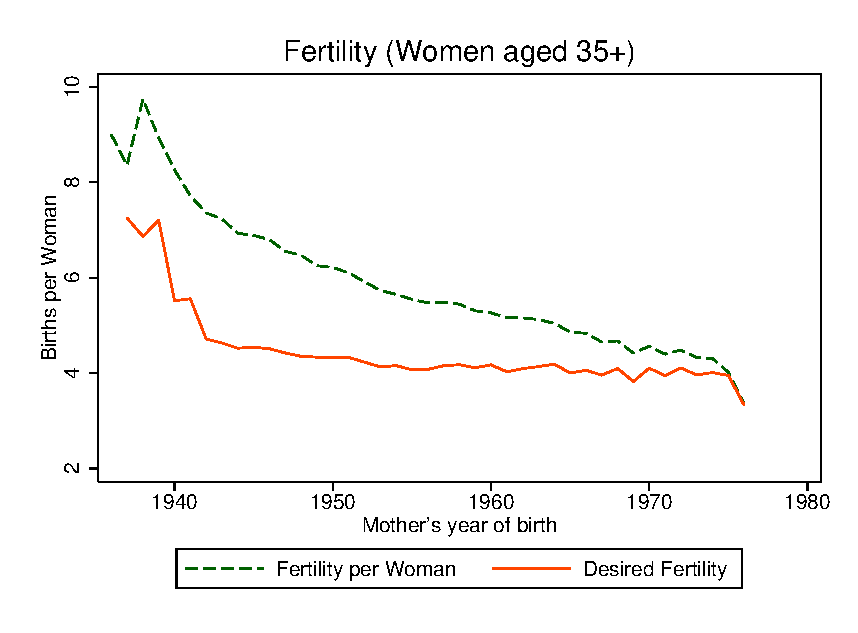
\includegraphics[scale=0.53]{\twinfolder/Figures/ferttrend_35_all.eps}
  \caption{Trends in Fertility}
  \label{TWINfig:fertrend}
\end{subfigure}%
\begin{subfigure}{.5\textwidth}
  \centering
  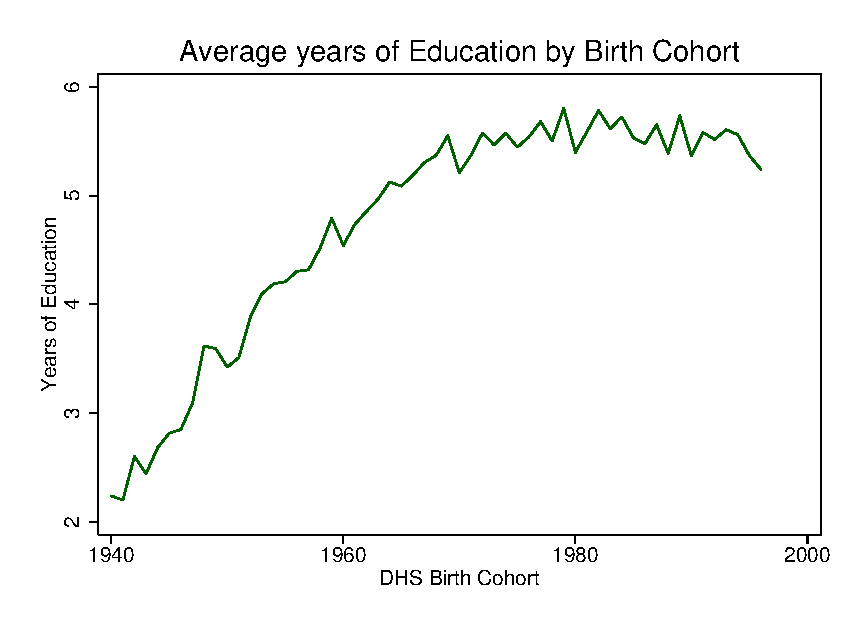
\includegraphics[scale=0.52]{\twinfolder/Figures/eductrend_all.eps}
  \caption{Trend in Education}
  \label{TWINfig:eductrend}
\end{subfigure}
\caption{Education and Fertility}
\label{TWINfig:trends}
\floatfoot{Note to figure \ref{TWINfig:trends}: Cohorts are made up of all individuals 
from the DHS who are over 35 years (for fertility), and over 15 years (for education).  
In each case the sample is restricted to those who have approximately completed fertility 
and education respectively.}
\end{figure}
\vspace{1cm}

\begin{figure}[htpb!]
\begin{center}
\caption{Proportion of Twins of All Births (USA)}
\label{TWINfig:bord}
\includegraphics[scale=0.92]{\twinfolder/Figures/USTwinFLE.eps} 
\end{center}
\end{figure}

\begin{figure}[htpb!]
\begin{center}
\caption{Twin Births and Total Fertility}
\label{TWINfig:births}
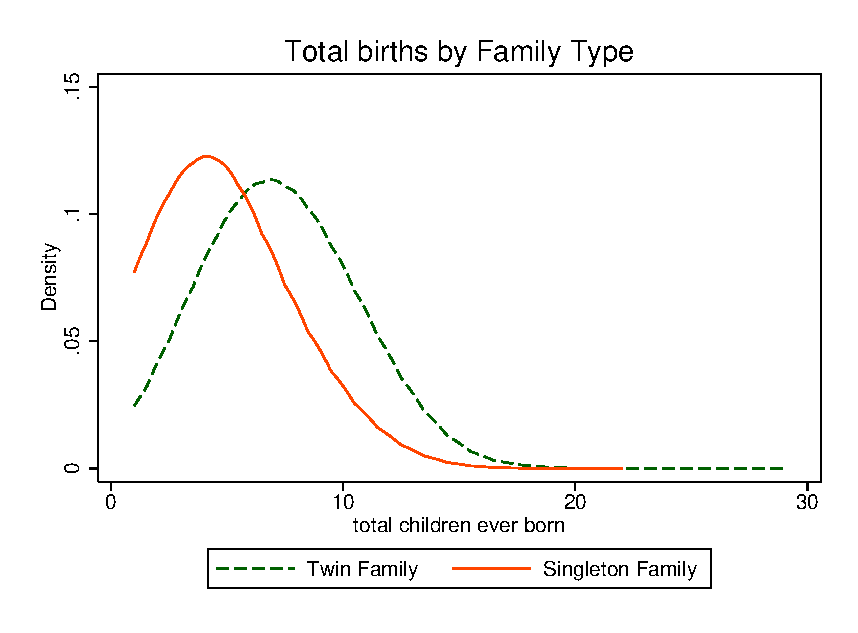
\includegraphics[scale=0.92]{\twinfolder/Figures/famsize.eps} 
\end{center}
\end{figure}

\begin{figure}[htpb!]
\begin{center}
\caption{Proportion of Twins by Birth Order}
\label{TWINfig:bord}
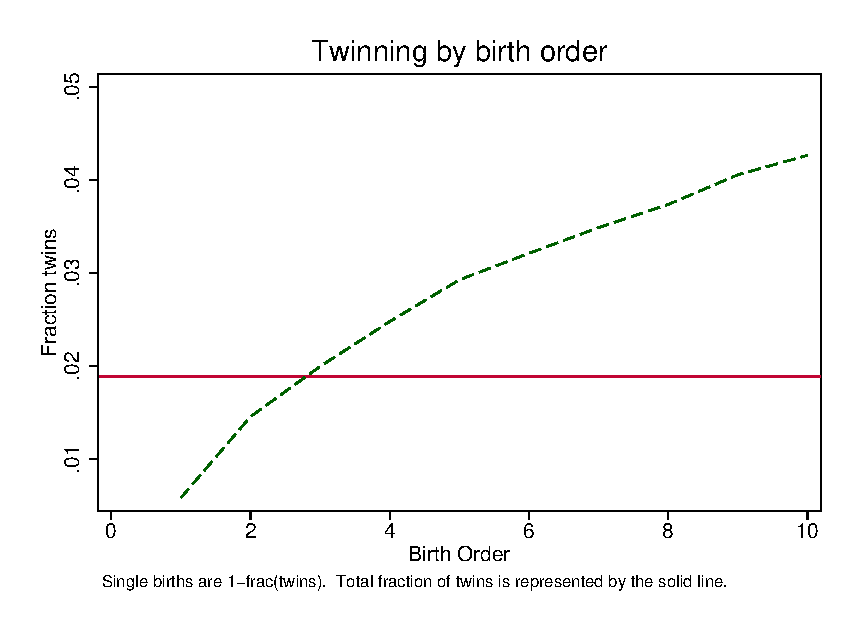
\includegraphics[scale=0.92]{\twinfolder/Figures/twinbybord.eps} 
\end{center}
\end{figure}

\begin{figure}[htpb!]
\begin{center}
\caption{Intra- and Inter-country trends: height and twinning}
\label{TWINfig:arrows}
\includegraphics[scale=0.86]{\twinfolder/Figures/height_country.eps} 
\end{center}
\end{figure}

%\begin{figure}[htpb!]
%\begin{center}
%\caption{Distribution of Ideal Family Size}
%\label{TWINfig:ideal}
%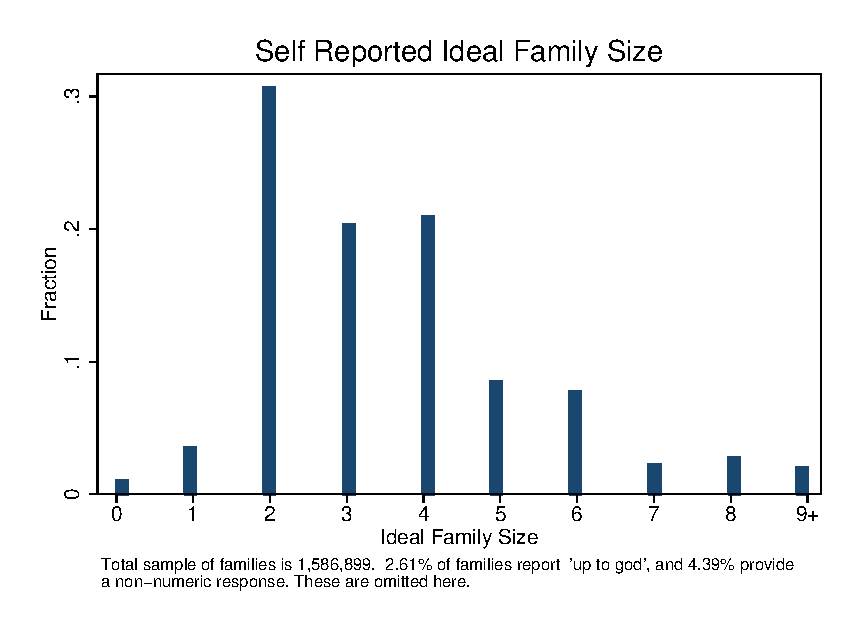
\includegraphics[scale=0.92]{\twinfolder/Figures/idealfamsize.eps} 
%\end{center}
%\end{figure}

%\begin{figure}[htpb!]
%\begin{center}
%\caption{Ideal and Actual Fertility}
%\label{TWINfig:idealactual}
%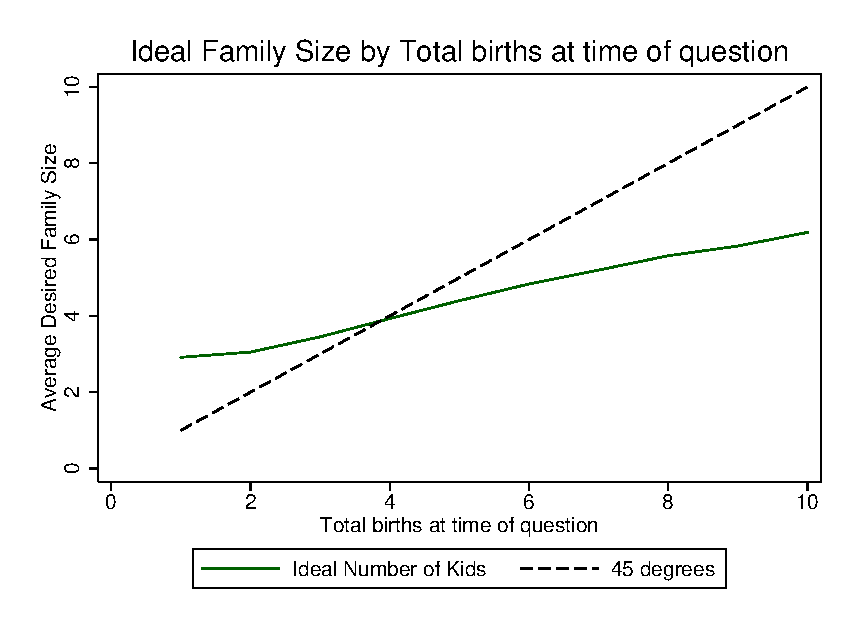
\includegraphics[scale=0.92]{\twinfolder/Figures/idealfam_fert.eps} 
%\end{center}
%\end{figure}

\begin{figure}[htpb!]
\begin{center}
\caption{Relaxing Strict Exogeneity (two plus)}
\label{TWINfig:ltz2}
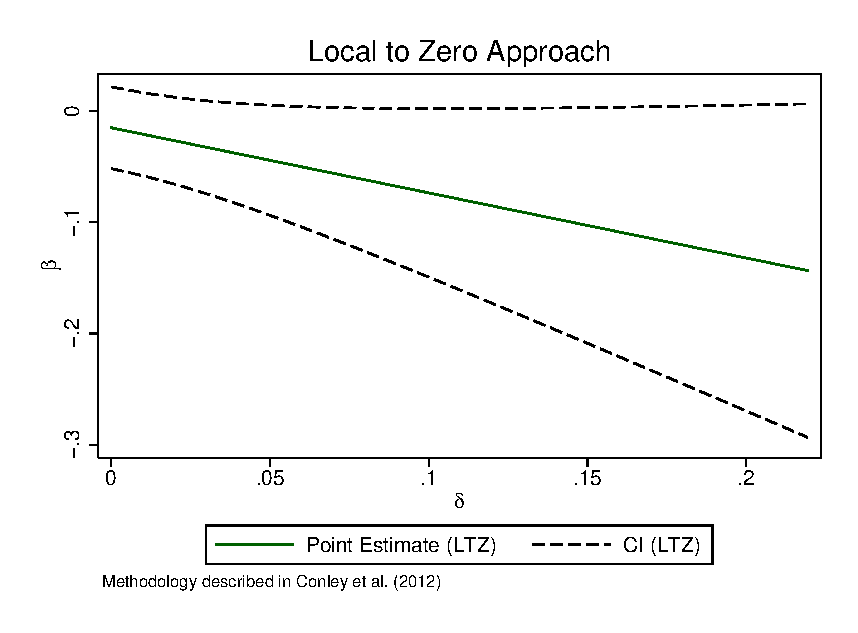
\includegraphics[scale=0.88]{\twinfolder/Figures/LTZ_two.eps}
\vspace{-8mm}
\floatfoot{Note to figure \ref{TWINfig:ltz2}: See note to Figure \ref{TWINfig:ltz3}}
\end{center}
\end{figure}

\begin{figure}[htpb!]
\begin{center}
\caption{Relaxing Strict Exogeneity (three plus)}
\label{TWINfig:ltz3}
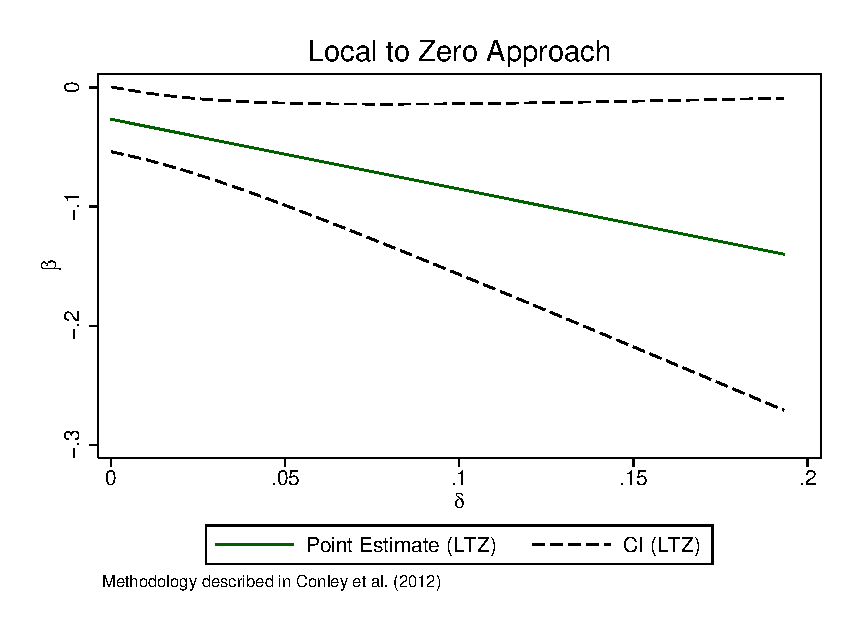
\includegraphics[scale=0.88]{\twinfolder/Figures/LTZ_three.eps} 
\floatfoot{Note to figure \ref{TWINfig:ltz3}: Confidence intervals and point estimates 
are calculated according to \citet{Conleyetal2012}.  Estimates reflect a range of priors 
regarding the validity of the exclusion restriction required to consistently estimate 
$\hat\beta_{fert}$ using twinning in a 2SLS framework.  The local to zero (LTZ) 
approach applied here assumes that $\gamma$, the sign on the instrument when included
in the first stage, is distributed $\gamma\sim U(0,\delta)$.  Further discussion 
is provided in the body of the text and table \ref{TWINtab:Conley}.}
\end{center}
\end{figure}




\clearpage
\section*{Tables}
\begin{table}[htpb!]\caption{Summary Statistics} 
\label{TWINtab:sumstats}\begin{center}\scalebox{0.99}{\begin{tabular}{lccccc}
\toprule \toprule 
&\multicolumn{2}{c}{Low Income}&\multicolumn{2}{c}{Middle Income}\\ 
\cmidrule(r){2-3} \cmidrule(r){4-5}
& Single & Twins & Single & Twins & All \\ \midrule 
\textsc{Fertility} & & & & & \\ 
Fertility&3.749&6.223&3.412&5.584&3.689\\
&(2.392)&(2.622)&(2.308)&(2.687)&(2.406)\\
Desired Family Size&4.193&5.328&3.380&4.190&3.921\\
&(2.530)&(2.885)&(2.130)&(2.555)&(2.440)\\
Fraction Twin & \multicolumn{2}{c}{  0.0200}& \multicolumn{2}{c}{  0.0179 } &  0.0191\\
& \multicolumn{2}{c}{(0.1402)}& \multicolumn{2}{c}{(0.1326)} & (0.1370)\\
Birth Order Twin & \multicolumn{2}{c}{   4.664}& \multicolumn{2}{c}{   4.016 }&   4.410\\
& \multicolumn{2}{c}{(2.465)}& \multicolumn{2}{c}{(2.374)}& (2.450)\\
\textsc{Mother's Characteristics}&&&&&\\ Age
&31.22&34.52&32.32&35.61&31.72\\
&(8.238)&(7.381)&(8.356)&(7.428)&(8.293)\\
Education&3.859&3.222&6.690&5.906&4.885\\
&(4.327)&(3.991)&(4.795)&(5.023)&(4.706)\\
Height&155.5&157.6&155.6&157.2&155.6\\
&(7.093)&(7.065)&(6.966)&(6.945)&(7.053)\\
BMI&21.90&22.50&25.90&26.63&23.39\\
&(4.027)&(4.175)&(5.118)&(5.512)&(4.867)\\
Pr(BMI)$<$18.5&0.175&0.125&0.0346&0.0276&0.122\\
&(0.380)&(0.331)&(0.183)&(0.164)&(0.327)\\
Actual Births$>$Desired&0.310&0.526&0.324&0.575&0.321\\
&(0.463)&(0.499)&(0.468)&(0.494)&(0.467)\\
\textsc{Children's Outcomes}&&&&&\\ Education (Years)
&3.660&3.204&5.445&5.043&4.446\\
&(3.576)&(3.293)&(3.867)&(3.760)&(3.810)\\
Education (Z-Score)&-0.00843&-0.0156&0.0119&-0.0428&0.000144\\
&(1.001)&(0.963)&(0.998)&(0.987)&(1.000)\\
No Education (Percent)&0.207&0.222&0.0649&0.0786&0.144\\
&(0.405)&(0.416)&(0.246)&(0.269)&(0.351)\\
Infant Mortality&0.0158&0.0917&0.00946&0.0497&0.0141\\
&(0.125)&(0.289)&(0.0968)&(0.217)&(0.118)\\
Child Mortality&0.0239&0.108&0.0122&0.0535&0.0199\\
&(0.153)&(0.310)&(0.110)&(0.225)&(0.140)\\
\midrule
Number of Countries & 39&39  & 28&28  & 67 \\
Number of Children &2,231,844 &45,654 &1,614,358 &29,430 & 3,921,286 \\
Number of Mothers &875,587 &12,908 &653,969 &8,605 & 1,586,899 \\
\midrule
\multicolumn{6}{p{13.2cm}}{\begin{footnotesize}\textsc{Notes:}  Group means are presented with standard deviation below in parenthesis.  Education is reported as total years attained, and Z-score presents educational attainment relative to country and cohort (mean 0, std deviation 1).  Infant mortality refers to the proportion of children who die before 1 year of age,  while child mortality refers to the proportion who die before 5 years.  Maternal height is reported in cm, and BMI is weight in kg over height in metres squared.  Summary statistics are for the full sample of 1,586,899
 mothers responding to any publicly available DHS survey.  For a full list of country and years of survey, see appendix table \ref{TWINtab:countries}.\end{footnotesize}} \\ \bottomrule \end{tabular}}\end{center}\end{table}


\begin{landscape}\begin{table}[htpb!]\caption{Fertility and the Twin Instrument: Literature} 
\label{TWINtab:Lit}\begin{center}\begin{tabular}{p{4cm}p{5cm}p{5cm}p{2cm}p{1.22cm}p{1.22cm}}
\toprule \toprule 
&&&&\multicolumn{2}{c}{Estimates}\\ \cmidrule(r){5-6}
Author & Data, Period & Controls Included & Sample & \ \ OLS & \ \ IV \\ \midrule 
(1) \citet{Blacketal2005} & 
Norway matched administrative files of
individuals aged 16-74 during 1986-2000,
(children $>$ 25 years). Outcome is 
completed years of education. & 
Age, parents' age, parents' education, 
sex. &  \begin{tabular}[t]{@{}l@{}} Two Plus \\ \\ Three Plus \\ \\ Four Plus \end{tabular}
& -0.060 (0.003) -0.076 (0.004) -0.059 (0.006)
& -0.038 (0.047) -0.016 (0.044) -0.024 (0.059) \\
&&&&& \\
(2) \citet{Caceres2006} & 
USA 1980 Census Five-Percent Public Use Micro Sample.
Children aged 6-16 years. Outcome (reported here) 
is an indicator of whether the child is behind his
or her cohort. & Age, state of residence, mother's
education, race, mother's age, sex. &
\begin{tabular}[t]{@{}l@{}} Two Plus \\ \\ Three Plus \end{tabular}
& 0.011 (0.000) 0.017 (0.001)
& 0.002 (0.003) 0.010 (0.006) \\
&&&&& \\
(3) \citet{Angristetal2010} & 
Israel 20\% public-use microdata samples
from 1995 and 1983 censuses, 18-60 year old respondents.
Outcome (reported here) is highest grade completed. &
Age, missing month of birth, mother's age, age at first birth
and age at immigration, mother's and father's 
place of birth, and census year. &
\begin{tabular}[t]{@{}l@{}} Two Plus \\ \\ Three Plus \end{tabular}
& -0.145 (0.005) -0.143 (0.005)
& 0.174 (0.166) 0.167 (0.117) \\
&&&&& \\
(4) \citet{Lietal2008} &
The 1 percent sample of the 1990 Chinese Population Census.
Subjects are 6-17 year olds with mothers who are 35 years of age or
younger.  Outcome (reported here) is years of schooling. 
& Child age, gender, ethnic group, birth order, and place of residence.
Parental age and educational level.
&
\begin{tabular}[t]{@{}l@{}} Two Plus \\ \\ Three Plus \end{tabular}
& -0.031 (-29.6)\textsuperscript{\dag} -0.038 (-21.4)\textsuperscript{\dag}
& 0.002 (0.18)\textsuperscript{\dag} -0.024 (-1.70)\textsuperscript{\dag} \\
&&&&& \\
(5) \citet{FitzsimonsMalde2014} &
Mexican Survey data (ENCASEH) from 1996-1999.  
Subjects are 12-17 year olds.  Outcome (reported here)
is years of schooling. & Parent's age, parents' years of schooling and
schooling dummies, birth spacing, household goods (rooms, land, water, etc).
&
\begin{tabular}[t]{@{}l@{}} Two Plus \\ \\ Three Plus \\ \\ Four Plus \end{tabular}
& -0.020 (0.001) -0.020 (0.001) -0.018 (0.002)
& -0.019 (0.015) 0.007 (0.025) -0.032 (0.036) \\
&&&&& \\




\end{tabular}\end{center}\end{table}\end{landscape}



\begin{landscape}\begin{table}[htpb!]\begin{center}\begin{tabular}{p{4cm}p{5cm}p{5cm}p{2cm}p{1.3cm}p{1.3cm}}
\midrule
&&&&\multicolumn{2}{c}{Estimates}\\ \cmidrule(r){5-6}
Author & Data, Period & Controls Included & Sample& \ \ OLS &\ \ IV \\ \midrule 
(6) \citet{RosenzweigZhang2009} & 
The Chinese Child Twins Survey (CCTS), 2002-2003.
Individuals selected from twins' (aged 7-18) and
non-twin households. Outcome (reported here) is years of schooling
 & 
Mother's age at time of birth, child gender and age.
 &  \begin{tabular}[t]{@{}l@{}} Reduced Form \\ \\ Reduced Form \\ + Bwt \end{tabular}
& \multicolumn{2}{c}{ 
\begin{tabular}[t]{@{}l@{}} -0.307 \\ (1.92)\textsuperscript{\dag} 
\\ -0.225 \\ (1.31)\textsuperscript{\dag} \end{tabular}} \\
&&&&& \\
(7) \citet{SouzaPonczek2012} & 
1991 Brazilian Census microdata, 10 and 20\% sample.
Children of 10-15 years, and 18-20 years old.  Outcome
reported here is years of school completed.
 & 
Child's gender, age and race controls,; mother and family head's 
years of schooling, and age.
&\begin{tabular}[t]{@{}l@{}} Two Plus \\ (M) \\ Two Plus \\ (F) \\ Three Plus \\ (M) \\ Three Plus \\ (F) \end{tabular}
& -0.233 (0.010) -0.277 (0.015) -0.230 (0.010) -0.283 (0.015)
& -0.137 (0.146) -0.372 (0.198) -0.060 (0.164) -0.634 (0.194) \\
&&&&& \\


\bottomrule 
\multicolumn{6}{p{20cm}}{\begin{footnotesize} Notes: Individual sources discussed further in the body of the text.  Estimates reported in each study are presented along with their standard errors in parenthesis. Parentheses
marked as \textsuperscript{\dag} contain the t-statistic rather than the standard error.\end{footnotesize}} 
\end{tabular}\end{center}\end{table}\end{landscape}



\begin{landscape}\begin{table}[htpb!] 
\caption{Probability of Giving Birth to Twins} \label{TWINtab:twinreg1} 
\begin{center}\begin{tabular}{lcccccc} \toprule \toprule 
&(1)&(2)&(3)&(4)&(5)&(6)\\
Twin$\times$100&All&\multicolumn{2}{c}{Income}&\multicolumn{2}{c}{Time}&Prenatal\\
 \cmidrule(r){3-4} \cmidrule(r){5-6} 
&&Low inc&Middle inc&1990-2013&1972-1989&\\\midrule
\begin{footnotesize}\end{footnotesize}&\begin{footnotesize}\end{footnotesize}&\begin{footnotesize}\end{footnotesize}&\begin{footnotesize}\end{footnotesize}&\begin{footnotesize}\end{footnotesize}&\begin{footnotesize}\end{footnotesize}&\begin{footnotesize}\end{footnotesize}\\
Age&0.491***&0.489***&0.498***&0.587***&0.168***&0.632***\\
&(0.026)&(0.033)&(0.045)&(0.030)&(0.064)&(0.040)\\
Age Squared&-0.006***&-0.006***&-0.007***&-0.008***&-0.000&-0.009***\\
&(0.000)&(0.001)&(0.001)&(0.001)&(0.001)&(0.001)\\
Age First Birth&-0.051***&-0.082***&-0.002&-0.050***&-0.051***&-0.041***\\
&(0.008)&(0.010)&(0.013)&(0.009)&(0.015)&(0.013)\\
Education (years)&0.027*&0.065***&-0.008&0.044**&-0.008&-0.071**\\
&(0.016)&(0.021)&(0.027)&(0.019)&(0.028)&(0.028)\\
Education squared&-0.001&-0.005**&0.001&-0.002&0.002&0.003\\
&(0.001)&(0.002)&(0.002)&(0.001)&(0.002)&(0.002)\\
Height&0.057***&0.056***&0.058***&0.063***&0.038***&0.059***\\
&(0.004)&(0.005)&(0.006)&(0.005)&(0.007)&(0.007)\\
BMI&0.050***&0.059***&0.043***&0.046***&0.056***&0.045***\\
&(0.006)&(0.008)&(0.008)&(0.007)&(0.009)&(0.011)\\
Prenatal (Doctor)&&&&&&0.917***\\
&&&&&&(0.129)\\
Prenatal (Nurse)&&&&&&0.076\\
&&&&&&(0.109)\\
Prenatal (None)&&&&&&-0.479***\\
&&&&&&(0.133)\\
&&&&&&\\R-squared&0.01&0.01&0.01&0.01&0.00&0.01\\
Observations &2271948&1430703&841245&1660253&611695&624990\\
\hline\hline\multicolumn{7}{p{14.3cm}}{\begin{footnotesize}\textsc{Notes:} All specifications include a full set of year of birth and  country dummies, and are estimated as linear probability models.  Twin is multiplied by 100 for presentation.  Height is measured in cm  and BMI is weight in kg divided by height in metres squared. l  Prenatal care variables are only recoreded for recent births.  As  such, column (6) is estimated only for that subset of births where  these observations are made.
$^{*}$p$<$0.1; $^{**}$p$<$0.05; $^{***}$p$<$0.01
 \end{footnotesize}}\\ \hline \normalsize \end{tabular}\end{center}\end{table}\end{landscape} 

\begin{table}[htpb!]
\caption{Test of hypothesis that women who bear twins have better prior health}\label{TWINtab:IMR}\begin{center}\begin{tabular}{lccc}
\toprule \toprule 
\textsc{Infant Mortality (per 100 births)}& Base & +S\&H & Observations \\ \midrule 
\begin{footnotesize}\end{footnotesize}& 
\begin{footnotesize}\end{footnotesize}& 
\begin{footnotesize}\end{footnotesize}& 
\begin{footnotesize}\end{footnotesize}\\ 
Treated (2+)\hspace{5mm}\hspace{5mm}\hspace{5mm}\hspace{5mm}\hspace{5mm}\hspace{5mm}&-2.065***&-2.110***&503785\\
&(0.212)&(0.213)&\\
Treated (3+)\hspace{5mm}&-4.619***&-4.632***&686931\\
&(0.201)&(0.201)&\\
Treated (4+)&-4.257***&-4.243***&676303\\
&(0.183)&(0.183)&\\
Treated (5+)&-3.353***&-3.324***&587919\\
&(0.183)&(0.183)&\\
\midrule\multicolumn{4}{p{12.1cm}}{\begin{footnotesize}\textsc{Notes:} The sample for these regressions consist of all children who have been entirely exposed to the risk of infant mortality (ie those over 1 year of age). Subsamples 2+, 3+, 4+ and 5+ are generated to allow comparison of children born at similar birth orders.  For a full description of these groups see the the body of the paper or notes to table \ref{TWINtab:IVAll}. Treated=1 refers to children who are born before a twin while Treated=0 refers to children of similar birth orders not born before a twin.  Base and S+H controls are described in table \ref{TWINtab:IVAll}.$^{*}$p$<$0.1; $^{**}$p$<$0.05; $^{***}$p$<$0.01 
\end{footnotesize}} \\ \bottomrule 
\end{tabular}\end{center}\end{table}
\begin{table}[htpb]
\caption{Probability of Giving Births to Twins (NHIS, USA)}
\begin{center}
\scalebox{0.64}{
\begin{tabular}{lcc} \toprule
&(1)&(2) \\
VARIABLES&Twin$\times$100&Twin$\times$100 \\ \midrule
&& \\
Mother's Height&0.0416**&0.0406** \\
&(0.0201)&(0.0201) \\
Mother's Education&0.0084&0.0033 \\
&(0.0162)&(0.0164) \\
Smokes (pre-Pregnancy)&-0.119&-0.0983 \\
&(0.115)&(0.116) \\
Mother's Age&0.0121&0.0108 \\
&(0.0446)&(0.0446) \\
Mother's Age$^2$ &-0.0008&-0.0008 \\
&(0.0006)&(0.0006) \\
Age First Birth &0.166***&0.164*** \\
&(0.0135)&(0.0136) \\
BMI &0.0123***&0.0130*** \\
&(0.0034)&(0.0034) \\
Mother Good Health&&0.203* \\
&&(0.116) \\
Mother Poor Health&&-0.00284 \\
&&(0.189) \\
Constant&-4.091***&-4.101*** \\
&(1.542)&(1.543) \\
&& \\
Observations&105,879&105,879 \\
R-squared&0.004&0.004 \\ \midrule
%\multicolumn{3}{ p{5cm} }{\begin{footnotesize}\textsc{Notes:} Standard errors in parentheses. *** p$<$0.01; ** p$<$0.05; * p$<$0.1\end{footnotesize}}\bottomrule
\end{tabular}}
\end{center}
\end{table}



\input{\twinfolder/Tables/Alderman.tex}
\input{\twinfolder/Tables/NepalRegs2.tex}

\begin{landscape}\begin{table}[!htbp] \centering 
\caption{OLS Estimates of the Q-Q Trade-off} 
 \vspace{4mm}\label{TWINtab:OLS} 
\begin{tabular}{lcccccc} \toprule \toprule 
&Base&+&+&Desired&Altonji&Altonji\\
&Controls&Socioec&Health&&Ratio 1&Ratio 2\\\midrule
\textsc{Panel A: All Countries}&&&&&&\\
Fertility &-0.115***&-0.0777***&-0.0751***&-0.0717***&2.083&1.882\\
&(0.000815)&(0.000776)&(0.000771)&(0.000838)&&\\
Fertility$\times$desire&&&&-0.00558***&&\\
&&&&(0.000495)&&\\
&&&&&&\\
Observations &1,334,874&1,334,874&1,334,874&1,334,874&&\\
R$^2$&0.094&0.161&0.167&0.168&&\\\midrule
\textsc{Panel B: Low Income}&&&&&&\\
Fertility &-0.110***&-0.0734***&-0.0712***&-0.0668***&2.005&1.835\\
&(0.00106)&(0.000988)&(0.000975)&(0.00107)&&\\
Fertility$\times$desire&&&&-0.00674***&&\\
&&&&(0.000608)&&\\
&&&&&&\\
Observations &831,476&831,476&831,476&831,476&&\\
R$^2$&0.091&0.171&0.181&0.182&&\\\midrule
\textsc{Panel C: Middle Income}&&&&&&\\
Fertility &-0.125***&-0.0875***&-0.0854***&-0.0839***&2.333&2.157\\
&(0.00128)&(0.00126)&(0.00126)&(0.00134)&&\\
Fertility$\times$desire&&&&-0.00266***&&\\
&&&&(0.000846)&&\\
&&&&&&\\
Observations &503,398&503,398&503,398&503,398&&\\
R$^2$&0.106&0.154&0.156&0.156&&\\\hline\hline
\multicolumn{7}{p{15.8cm}}{\begin{footnotesize}\textsc{Notes:} Base controls consist of child gender, mother's age and age squared mother's age at first birth, child age, country, and year of birth dummies.  Socioeconomic augments `Base' to include mother's education and education squared, and Health includes mother's height and BMI. ``Desire'' takes 1 if the child is born before the family reaches it's desired size, and 0 if the child is born after the desired size is reached. The \citet{Altonjietal2005} ratio determines how important unobservable factors must be compared with included observables to imply that the true effect of fertilty on educational attainment is equal to zero.  Ratio 1 compares no controls to socioeconomic controls, while ratio 2 compares no controls to socioeconomic and health controls. Standard errors are clustered at the level of the mother.
$^{*}$p$<$0.1; $^{**}$p$<$0.05; $^{***}$p$<$0.01\end{footnotesize}}\\  
\bottomrule \normalsize\end{tabular}\end{table}\end{landscape} 

\begin{table}[htpb!]\caption{Principal IV Results}
\label{TWINtab:IVAll}
\begin{center}\scalebox{0.55}{
\begin{tabular}{lcccp{2mm}cccp{2mm}ccc}
\toprule \toprule 
&\multicolumn{3}{c}{2+}&&\multicolumn{3}{c}{3+}&&\multicolumn{3}{c}{4+}\\ \cmidrule(r){2-4} \cmidrule(r){6-8} \cmidrule(r){10-12} 
\textsc{School Z-Score}&Base&+H&+S\&H&&Base&+H&+S\&H&&Base&+H&+S\&H\\ \midrule 
\begin{footnotesize}\end{footnotesize}& 
\begin{footnotesize}\end{footnotesize}& 
\begin{footnotesize}\end{footnotesize}& 
\begin{footnotesize}\end{footnotesize}& 
\begin{footnotesize}\end{footnotesize}& 
\begin{footnotesize}\end{footnotesize}& 
\begin{footnotesize}\end{footnotesize}& 
\begin{footnotesize}\end{footnotesize}& 
\begin{footnotesize}\end{footnotesize}& 
\begin{footnotesize}\end{footnotesize}& 
\begin{footnotesize}\end{footnotesize}& 
\begin{footnotesize}\end{footnotesize}\\ 
\multicolumn{12}{l}{\textbf{All}}\\ 
Fertility&0.006&-0.026&-0.026&&-0.004&-0.036&-0.038*&&-0.017&-0.036&-0.035*\\
&(0.029)&(0.027)&(0.026)&&(0.024)&(0.022)&(0.021)&&(0.025)&(0.023)&(0.021)\\
\begin{footnotesize}\end{footnotesize}&\begin{footnotesize}\end{footnotesize}&\begin{footnotesize}\end{footnotesize}&\begin{footnotesize}\end{footnotesize}&\begin{footnotesize}\end{footnotesize}&\begin{footnotesize}\end{footnotesize}&\begin{footnotesize}\end{footnotesize}&\begin{footnotesize}\end{footnotesize}&\begin{footnotesize}\end{footnotesize}&\begin{footnotesize}\end{footnotesize}&\begin{footnotesize}\end{footnotesize}&\begin{footnotesize}\end{footnotesize}\\Observations&249536&249536&249536&&375987&375987&375987&&385389&385389&385389\\
\multicolumn{12}{l}{\textbf{Low-Income}}\\ 
Fertility&0.035&0.008&0.012&&0.016&-0.016&-0.027&&-0.011&-0.031&-0.024\\
&(0.034)&(0.032)&(0.031)&&(0.030)&(0.028)&(0.026)&&(0.029)&(0.027)&(0.025)\\
\begin{footnotesize}\end{footnotesize}&\begin{footnotesize}\end{footnotesize}&\begin{footnotesize}\end{footnotesize}&\begin{footnotesize}\end{footnotesize}&\begin{footnotesize}\end{footnotesize}&\begin{footnotesize}\end{footnotesize}&\begin{footnotesize}\end{footnotesize}&\begin{footnotesize}\end{footnotesize}&\begin{footnotesize}\end{footnotesize}&\begin{footnotesize}\end{footnotesize}\\Observations&149602&149602&149602&&232371&232371&232371&&246622&246622&246622\\
\multicolumn{12}{l}{\textbf{Middle-Income}}\\ 
Fertility&-0.065&-0.087*&-0.093**&&-0.046&-0.079**&-0.067*&&-0.027&-0.048&-0.054\\
&(0.053)&(0.049)&(0.047)&&(0.040)&(0.036)&(0.035)&&(0.043)&(0.040)&(0.037)\\
\begin{footnotesize}\end{footnotesize}&\begin{footnotesize}\end{footnotesize}&\begin{footnotesize}\end{footnotesize}&\begin{footnotesize}\end{footnotesize}&\begin{footnotesize}\end{footnotesize}&\begin{footnotesize}\end{footnotesize}&\begin{footnotesize}\end{footnotesize}&\begin{footnotesize}\end{footnotesize}&\begin{footnotesize}\end{footnotesize}&\begin{footnotesize}\end{footnotesize}\\Observations&99934&99934&99934&&143616&143616&143616&&138767&138767&138767\\
\multicolumn{12}{l}{\textbf{Adjusted Fertility}}\\ 
Fertility&0.017&-0.052&-0.055&&-0.013&-0.073*&-0.077*&&-0.033&-0.068&-0.066*\\
&(0.065)&(0.056)&(0.054)&&(0.047)&(0.043)&(0.040)&&(0.045)&(0.042)&(0.039)\\
\begin{footnotesize}\end{footnotesize}&\begin{footnotesize}\end{footnotesize}&\begin{footnotesize}\end{footnotesize}&\begin{footnotesize}\end{footnotesize}&\begin{footnotesize}\end{footnotesize}&\begin{footnotesize}\end{footnotesize}&\begin{footnotesize}\end{footnotesize}&\begin{footnotesize}\end{footnotesize}&\begin{footnotesize}\end{footnotesize}&\begin{footnotesize}\end{footnotesize}\\Observations&249505&249505&249505&&375957&375957&375957&&385363&385363&385363\\
\multicolumn{12}{l}{\textbf{Twins and Pre-Twins}}\\ 
Fertility&-0.021&-0.073***&-0.078***&&-0.019&-0.062***&-0.067***&&-0.018&-0.039**&-0.046**\\
&(0.024)&(0.021)&(0.020)&&(0.020)&(0.018)&(0.018)&&(0.021)&(0.019)&(0.018)\\
\begin{footnotesize}\end{footnotesize}&\begin{footnotesize}\end{footnotesize}&\begin{footnotesize}\end{footnotesize}&\begin{footnotesize}\end{footnotesize}&\begin{footnotesize}\end{footnotesize}&\begin{footnotesize}\end{footnotesize}&\begin{footnotesize}\end{footnotesize}&\begin{footnotesize}\end{footnotesize}&\begin{footnotesize}\end{footnotesize}&\begin{footnotesize}\end{footnotesize}\\Observations&488815&488815&488815&&563177&563177&563177&&523197&523197&523197\\
\bottomrule
\end{tabular}}\end{center}\end{table}

\begin{table}[htpb!]\caption{NHIS Estimates (USA): Education and Health}
\label{TWINtab:NHISAll}
\begin{center}
\scalebox{0.52}{
\begin{tabular}{lcccp{2mm}cccp{2mm}ccc}
\toprule \toprule 
&\multicolumn{3}{c}{2+}&&\multicolumn{3}{c}{3+}&&\multicolumn{3}{c}{4+}\\ \cmidrule(r){2-4} \cmidrule(r){6-8} \cmidrule(r){10-12} 
&Base&+H&+S\&H&&Base&+H&+S\&H&&Base&+H&+S\&H\\ \midrule 
\begin{footnotesize}\end{footnotesize}& 
\begin{footnotesize}\end{footnotesize}& 
\begin{footnotesize}\end{footnotesize}& 
\begin{footnotesize}\end{footnotesize}& 
\begin{footnotesize}\end{footnotesize}& 
\begin{footnotesize}\end{footnotesize}& 
\begin{footnotesize}\end{footnotesize}& 
\begin{footnotesize}\end{footnotesize}& 
\begin{footnotesize}\end{footnotesize}& 
\begin{footnotesize}\end{footnotesize}& 
\begin{footnotesize}\end{footnotesize}& 
\begin{footnotesize}\end{footnotesize}\\ 
\multicolumn{12}{l}{\textbf{OLS}}\\ 
School Z-Score&-0.043***&-0.033***&-0.027***&&-0.036***&-0.028***&-0.020**&&-0.010&-0.004&0.002\\
&(0.005)&(0.006)&(0.006)&&(0.008)&(0.009)&(0.009)&&(0.018)&(0.018)&(0.018)-\\
Excellent Health&-0.012***&-0.005***&-0.004*&&-0.018***&-0.010***&-0.008***&&-0.028***&-0.019***&-0.017***\\
&(0.002)&(0.002)&(0.002)&&(0.004)&(0.003)&(0.003)&&(0.006)&(0.005)&(0.005)\\

\begin{footnotesize}\end{footnotesize}&\begin{footnotesize}\end{footnotesize}&\begin{footnotesize}\end{footnotesize}&\begin{footnotesize}\end{footnotesize}&\begin{footnotesize}\end{footnotesize}&\begin{footnotesize}\end{footnotesize}&\begin{footnotesize}\end{footnotesize}&\begin{footnotesize}\end{footnotesize}&\begin{footnotesize}\end{footnotesize}&\begin{footnotesize}\end{footnotesize}&\begin{footnotesize}\end{footnotesize}&\begin{footnotesize}\end{footnotesize}\\
\multicolumn{12}{l}{\textbf{IV}}\\ 
School Z-Score&-0.064&-0.074&-0.077&&-0.027&-0.037&-0.036&&-0.094&-0.099&-0.113\\
&(0.063)&(0.059)&(0.058)&&(0.065)&(0.064)&(0.065)&&(0.152)&(0.155)&(0.150)\\

Excellent Health&0.013&0.022&0.019&&-0.016&-0.054*&-0.055*&&0.057&0.017&0.006\\
&(0.025)&(0.020)&(0.020)&&(0.038)&(0.031)&(0.031)&&(0.058)&(0.054)&(0.052)\\
\begin{footnotesize}\end{footnotesize}&\begin{footnotesize}\end{footnotesize}&\begin{footnotesize}\end{footnotesize}&\begin{footnotesize}\end{footnotesize}&\begin{footnotesize}\end{footnotesize}&\begin{footnotesize}\end{footnotesize}&\begin{footnotesize}\end{footnotesize}&\begin{footnotesize}\end{footnotesize}&\begin{footnotesize}\end{footnotesize}&\begin{footnotesize}\end{footnotesize}&\begin{footnotesize}\end{footnotesize}&\begin{footnotesize}\end{footnotesize}\\
\multicolumn{12}{l}{\textbf{Descriptives}}\\ 
School Z-Score&-0.0233&&&&-0.0363&&&&-0.0628&&\\
&(0.993)&&&&(1.041)&&&&(1.086)&&\\
Excellent Health&0.533&&&&0.511&&&&0.490&&\\
&(0.499)&&&&(0.500)&&&&(0.500)&&\\
\begin{footnotesize}\end{footnotesize}&\begin{footnotesize}\end{footnotesize}&\begin{footnotesize}\end{footnotesize}&\begin{footnotesize}\end{footnotesize}&\begin{footnotesize}\end{footnotesize}&\begin{footnotesize}\end{footnotesize}&\begin{footnotesize}\end{footnotesize}&\begin{footnotesize}\end{footnotesize}&\begin{footnotesize}\end{footnotesize}&\begin{footnotesize}\end{footnotesize}&\begin{footnotesize}\end{footnotesize}&\begin{footnotesize}\end{footnotesize}\\ 
Observations & 75,902 &	75,902 &	75,902 &&	57,413 &	57,413 &	57,413 &&	26,128 &	26,128 &	26,128 \\
Joint F-test Educ &&164.5&64.7&&&101.3&39.6&&&38.0&7.7\\
Joint F-test Health &&34469.6&163.9&&&15335.6&28.4&&&5276.4&17.1\\
\midrule\multicolumn{12}{p{20.6cm}}{\begin{footnotesize}\textsc{Notes:}  
Each cell presents the coefficient of interest from a regression using NHIS survey data (2002-2014). Base controls include child age FE (in months), mother's age, and mother's age at first birth 
plus race dummies for child and mother.  First stage omitted for clarity (generally all around 0.7).  Standard errors are clustered by mother.$^{*}$p$<$0.1; $^{**}$p$<$0.05; $^{***}$p$<$0.01. 
\end{footnotesize}} \\ \bottomrule 
\end{tabular}}\end{center}\end{table}


\begin{table}[htpb!]\caption{`Plausibly Exogenous' Bounds} 
\label{TWINtab:Conley}\begin{center}\begin{tabular}{lcccc}
\toprule \toprule 
&\multicolumn{2}{c}{UCI: $\gamma\in [0,\delta]$}&\multicolumn{2}{c}{LTZ: $\gamma \sim U(0,\delta)$}\\ 
\cmidrule(r){2-3} \cmidrule(r){4-5}
&Lower Bound&Upper Bound&Lower Bound&Upper Bound\\
Two Plus&-0.1860&0.0195&-0.1613&0.0011\\
Three Plus&-0.1710&0.0025&-0.1528&-0.0116\\
Four Plus&-0.1539&-0.0067&-0.1391&-0.0194\\
Five Plus&-0.1373&0.0277&-0.1215&0.0143\\
\midrule\multicolumn{5}{p{11.6cm}}{\begin{footnotesize}\textsc{Notes:} This table presents upper and lower bounds of a 95\% confidence interval for the effects of family size on (standardised) children's education attainment. These are estimated by the methodology of \citet{Conleyetal2012}  under various priors about the direct effect that being from a twin family has on educational outcomes ($\gamma$). In the UCI (union of confidence interval) approach, it is assumed the true $\gamma\in[0,\delta]$, while in the LTZ (local to zero) approach it is assumed that $\gamma\sim U(0,\delta)$.  In each case $\delta$ is estimated by including twinning in the first stage  equation and observing the effect size $\hat\gamma$.  Estimated $\hat\gamma$'s are (respectively for two plus to five plus):   0.1088, 0.0983, 0.0826, 0.0929.\end{footnotesize}}  
\\ \bottomrule \end{tabular}\end{center}\end{table} 



\clearpage


\bibliography{./BiBBase1}

\newpage
\appendix
\section*{Appendices}
\section{Data Appendix}
Discuss: DHS, NHIS, USA registry data, Spain registry data, Chile survey, 

\newpage
\end{spacing}

\section{Appendix Tables}
\setcounter{table}{0}
\renewcommand{\thetable}{A\arabic{table}}

\begin{table}[htpb!]
\caption{United States Birth Registry (Administrative 2003-2012)}
\begin{center}
\scalebox{0.54}{
\begin{tabular}{lcccc} \hline
 & (1) & (2) & (3) & (4) \\
VARIABLES & twin100 & twin100 & twin100 & twin100 \\ \hline
\vspace{4pt} & \begin{footnotesize}\end{footnotesize} & \begin{footnotesize}\end{footnotesize} & \begin{footnotesize}\end{footnotesize} & \begin{footnotesize}\end{footnotesize} \\
africanAmerican & 0.554*** & 0.437*** & 0.437*** & 0.331*** \\
\vspace{4pt} & \begin{footnotesize}(0.00911)\end{footnotesize} & \begin{footnotesize}(0.0142)\end{footnotesize} & \begin{footnotesize}(0.0142)\end{footnotesize} & \begin{footnotesize}(0.0143)\end{footnotesize} \\
otherRace & 0.0433*** & 0.135*** & 0.135*** & -0.680*** \\
\vspace{4pt} & \begin{footnotesize}(0.00886)\end{footnotesize} & \begin{footnotesize}(0.0148)\end{footnotesize} & \begin{footnotesize}(0.0148)\end{footnotesize} & \begin{footnotesize}(0.0200)\end{footnotesize} \\
meducSecondary & 0.00124 & 0.0124 & 0.0124 & 0.810*** \\
\vspace{4pt} & \begin{footnotesize}(0.00881)\end{footnotesize} & \begin{footnotesize}(0.0159)\end{footnotesize} & \begin{footnotesize}(0.0159)\end{footnotesize} & \begin{footnotesize}(0.0203)\end{footnotesize} \\
meducTertiary & 1.124*** & 1.110*** & 1.110*** & 2.063*** \\
\vspace{4pt} & \begin{footnotesize}(0.00930)\end{footnotesize} & \begin{footnotesize}(0.0158)\end{footnotesize} & \begin{footnotesize}(0.0158)\end{footnotesize} & \begin{footnotesize}(0.0209)\end{footnotesize} \\
tobaccoUse & -0.327*** & -0.424*** & -0.424*** & -0.422*** \\
\vspace{4pt} & \begin{footnotesize}(0.0126)\end{footnotesize} & \begin{footnotesize}(0.0181)\end{footnotesize} & \begin{footnotesize}(0.0181)\end{footnotesize} & \begin{footnotesize}(0.0182)\end{footnotesize} \\
alcoholUse &  & -1.233*** & -1.233*** & -1.182*** \\
\vspace{4pt} & \begin{footnotesize}\end{footnotesize} & \begin{footnotesize}(0.0648)\end{footnotesize} & \begin{footnotesize}(0.0648)\end{footnotesize} & \begin{footnotesize}(0.0651)\end{footnotesize} \\
anemia &  &  &  & -1.349*** \\
\vspace{4pt} & \begin{footnotesize}\end{footnotesize} & \begin{footnotesize}\end{footnotesize} & \begin{footnotesize}\end{footnotesize} & \begin{footnotesize}(0.0335)\end{footnotesize} \\
diabetes &  &  &  & -0.408*** \\
\vspace{4pt} & \begin{footnotesize}\end{footnotesize} & \begin{footnotesize}\end{footnotesize} & \begin{footnotesize}\end{footnotesize} & \begin{footnotesize}(0.0280)\end{footnotesize} \\
chyper &  &  &  & -0.883*** \\
\vspace{4pt} & \begin{footnotesize}\end{footnotesize} & \begin{footnotesize}\end{footnotesize} & \begin{footnotesize}\end{footnotesize} & \begin{footnotesize}(0.0528)\end{footnotesize} \\
phyper &  &  &  & -4.128*** \\
\vspace{4pt} & \begin{footnotesize}\end{footnotesize} & \begin{footnotesize}\end{footnotesize} & \begin{footnotesize}\end{footnotesize} & \begin{footnotesize}(0.0267)\end{footnotesize} \\
eclamp &  &  &  & -5.686*** \\
\vspace{4pt} & \begin{footnotesize}\end{footnotesize} & \begin{footnotesize}\end{footnotesize} & \begin{footnotesize}\end{footnotesize} & \begin{footnotesize}(0.0896)\end{footnotesize} \\
Constant & 5.461*** & 5.326*** & 5.326*** & 32.75*** \\
 & \begin{footnotesize}(0.0525)\end{footnotesize} & \begin{footnotesize}(0.0806)\end{footnotesize} & \begin{footnotesize}(0.0806)\end{footnotesize} & \begin{footnotesize}(0.293)\end{footnotesize} \\
\vspace{4pt} & \begin{footnotesize}\end{footnotesize} & \begin{footnotesize}\end{footnotesize} & \begin{footnotesize}\end{footnotesize} & \begin{footnotesize}\end{footnotesize} \\
Observations & 38,910,055 & 16,605,619 & 16,605,619 & 12,219,256 \\
 $R^2$ & 0.008 & 0.008 & 0.008 & 0.012 \\ \hline
\multicolumn{5}{c}{\begin{footnotesize} Standard errors in parentheses\end{footnotesize}} \\
\multicolumn{5}{c}{\begin{footnotesize} *** p$<$0.01, ** p$<$0.05, * p$<$0.1\end{footnotesize}} \\
\end{tabular}}
\end{center}
\end{table}

\begin{table}[htpb!] 
\caption{Probability of Giving Birth to Twins (Chile)} 
\label{TWINtab:Chile} 
\begin{center}\begin{tabular}{lclc} \toprule \toprule 
&(1)&&\\
Twin$\times$100&&&\\\midrule
\multicolumn{2}{l}{\textsc{Pre-Pregnancy}}&\multicolumn{2}{l}{\textsc{Pregnancy}}\\\begin{footnotesize}\end{footnotesize}&\begin{footnotesize}\end{footnotesize}&\begin{footnotesize}\end{footnotesize}&\begin{footnotesize}\end{footnotesize}\\
Income p.c.&-0.006&Smoked&-0.573\\
&	(0.011)
&&	(0.416)
\\
Income p.c. squared&0.000&Drugs (infrequent)&-0.119\\
&	(0.000)
&&	(1.646)
\\
Secondary Education&0.142&Drugs (frequent)&-1.872***\\
&	(0.300)
&&	(0.344)
\\
Tertiary Education&1.507***&Alcohol (infrequent)&-0.002\\
&	(0.583)
&&	(0.570)
\\
Low Weight&-0.589&Alcohol (frequent)&-1.891***\\
&	(0.471)
&&	(0.290)
\\
Obese&-1.997***&No Check-ups&-1.031\\
&	(0.766)
&&	(0.966)
\\
Mother's Age&0.410***&Hospital Birth&0.939***\\
&	(0.133)
&&	(0.344)
\\
Mother's Age Squared&-0.007***&Diabetes&-0.255\\
&	(0.002)
&&	(0.505)
\\
Indigenous&-1.027***&Depression&0.031\\
&	(0.395)
&&	(0.416)
\\
&&&\\
Observations&14268&R-squared&0.00\\
\midrule\multicolumn{4}{p{11cm}}{\begin{footnotesize}\textsc{Notes:} Data comes from the Encuesta Longitudinal de Primera Infancia (ELPI) from Chile. Education at each level are dummy variables, primary education is the omitted base. Regional controls and child age fixed effects are omitted for clarity. Heteroscedasticity robust standard errors are presented in parenthesis.$^{*}$p$<$0.1; $^{**}$p$<$0.05; $^{***}$p$<$0.01\end{footnotesize}}\\ \hline \normalsize \end{tabular}\end{center}\end{table}

\begin{table}[htpb!] 
\caption{Probability of Giving Birth to Twins (Scotland)} 
\label{TWINtab:Scotland} 
\begin{center}\begin{tabular}{lclc} \toprule \toprule 
&(1)&&\\
Twin$\times$100&&&\\\midrule
\multicolumn{2}{l}{\textsc{Pre-Pregnancy}}&\multicolumn{2}{l}{\textsc{Pregnancy}}\\\begin{footnotesize}\end{footnotesize}&\begin{footnotesize}\end{footnotesize}&\begin{footnotesize}\end{footnotesize}&\begin{footnotesize}\end{footnotesize}\\
Deprivation Index (Quintile 2)&-1.628**
&Smoker&0.001
\\
&(0.958)
&&(0.669)
\\
Deprivation Index (Quintile 3)&-0.188
&Previous Smoker&1.717**
\\
&(0.967)
&&(0.877)
\\
Deprivation Index (Quintile 4)&-0.421
&Alcohol (1-2 per week)&-4.498*
\\
&(0.934)
&&(1.935)
\\
Deprivation Index (Quintile 5)&-1.132
&Alcohol (3+ per week)&-3.030*
\\
&(0.920)
&&(1.543)
\\
Height&0.306***
&Overweight&-0.092
\\
&(0.044)
&&(0.643)
\\
Married&3.272***
&Obese&1.350**
\\
&(0.878)
&&(0.746)
\\
Age&-0.337
&Diabetes&-0.188
\\
&(0.400)
&&(0.967)
\\
Age Squared&0.020***
&&\\
&(0.007)
&&\\
&&&\\
Observations&193254
&R-squared&0.01\\
\midrule\multicolumn{4}{p{11cm}}{\begin{footnotesize}\textsc{Notes:} Data comes from the ADD NOTE HERE!.$^{*}$p$<$0.1; $^{**}$p$<$0.05; $^{***}$p$<$0.01\end{footnotesize}}\\ \hline \normalsize \end{tabular}\end{center}\end{table}

\begin{table}[htpb!] 
\caption{Probability of Giving Birth to Twins (Sweden Birth Registry)} \label{TWINtab:twinregS} 
\begin{center}
\scalebox{0.64}{
\begin{tabular}{lccc} \toprule \toprule 
&(1)&(2)&(3)\\
Twin*100&All&\multicolumn{2}{c}{Time}\\
 \cmidrule(r){3-4} 
&&1991-2010&1983-1990\\\midrule
\begin{footnotesize}\end{footnotesize}&\begin{footnotesize}\end{footnotesize}&\begin{footnotesize}\end{footnotesize}&\begin{footnotesize}\end{footnotesize}\\
Age&0.257***&0.483***&0.277***\\
&(0.031)&(0.047)&(0.040)\\
Age Squared&-0.002***&-0.005***&-0.003***\\
&(0.001)&(0.001)&(0.001)\\
Education (years)&0.014&0.011&-0.013\\
&(0.009)&(0.014)&(0.012)\\
Height&0.038***&0.047***&0.019***\\
&(0.003)&(0.003)&(0.004)\\
Smoked&0.252***&0.237***&0.208***\\
&(0.045)&(0.069)&(0.056)\\
Alcohol&0.160&-2.381***&0.137\\
&(1.176)&(0.414)&(1.192)\\
&&&\\R-squared&0.01&0.01&0.01\\
Observations &1,628,737&1,098,076&530,661\\
\hline\hline\multicolumn{4}{p{8.3cm}}{\begin{footnotesize}\textsc{Notes:} Conditional on birth cohorts and marriage status FEs.  Linear probability estimates.  Standard errors in parenthesis are clustered at the level of the mother.
$^{*}$p$<$0.1; $^{**}$p$<$0.05; $^{***}$p$<$0.01
 \end{footnotesize}}\\ \hline \normalsize \end{tabular}}\end{center}\end{table} 


\input{\twinfolder/Tables/LeeBounds.tex}
\input{\twinfolder/Tables/TwinRegs/USfdeaths.tex}
\begin{table}
\caption{Twins, Miscarriage and Maternal Health (Administrative Data from Spain)}
\begin{center}
\scalebox{0.5}{
\begin{tabular}{lc}
\hline
VARIABLES	&	Fetal Death*100 \\	\hline
	&	(1)	\\
Primary	&	  -0.60179***	\\
	&	 (0.01456)	\\
Primary*Twin	&	   -0.6618***	\\
	&	 (0.20926)	\\
Secondary	&	  -0.71998*	\\
	&	  (0.0151)	\\
Secondary*Twin	&	  -0.55901***	\\
	&	 .0020978	\\
Tertiary	&	  -0.80019***	\\
	&	(0.01582)	\\
Tertiary*Twin	&	  -0.65091***	\\
	&	(0.20866)	\\
Immigration	&	  -0.07223***	\\
	&	 (0.0171)	\\
Immigration*Twin	&	  0.22871	\\
	&	(0.29614)	\\
Citm	&	  -0.00321	\\
	&	(0.01584)	\\
Citm*Twin	&	  0.09566	\\
	&	 (0.26876)	\\
Married	&	  -0.07354***	\\
	&	 (0.00759)	\\
Married*Twin	&	  -0.08978	\\
	&	 (0.11893)	\\
No Father	&	0.68626***	\\
	&	 (0.23825)	\\
No Father*Twin	&	3.25232	\\
	&	(4.09309)	\\
Constant	&	-1.35966***	\\
	&	(0.33674)	\\
	& \\
	Obs & 2869329 \\
	$R^2$ & 0.0044 \\ \hline
	\multicolumn{2}{p{5cm}}{Note: Spanish administrative births: 2007-2012.}
\end{tabular}}
\end{center}
\end{table}


\input{\twinfolder/Tables/OLSPlus.tex}
\begin{landscape}\begin{table}[htpb!]\caption{First Stage Results} 
\label{TWINtab:FS}\begin{center}\begin{tabular}{lcccp{2mm}cccp{2mm}ccc}
\toprule \toprule 
&\multicolumn{3}{c}{2+}&&\multicolumn{3}{c}{3+}&&\multicolumn{3}{c}{4+}\\ \cmidrule(r){2-4} \cmidrule(r){6-8} \cmidrule(r){10-12} 
\textsc{Fertility}&Base&+H&+S\&H&&Base&+H&+S\&H&&Base&+H&+S\&H\\ \midrule 
\begin{footnotesize}\end{footnotesize}& 
\begin{footnotesize}\end{footnotesize}& 
\begin{footnotesize}\end{footnotesize}& 
\begin{footnotesize}\end{footnotesize}& 
\begin{footnotesize}\end{footnotesize}& 
\begin{footnotesize}\end{footnotesize}& 
\begin{footnotesize}\end{footnotesize}& 
\begin{footnotesize}\end{footnotesize}& 
\begin{footnotesize}\end{footnotesize}& 
\begin{footnotesize}\end{footnotesize}\\ 
\multicolumn{12}{l}{\textbf{All}}\\ 
Twin&0.776***&0.821***&0.822***&&0.794***&0.827***&0.826***&&0.840***&0.859***&0.861***\\
&(0.031)&(0.029)&(0.028)&&(0.027)&(0.027)&(0.026)&&(0.027)&(0.027)&(0.026)\\
\begin{footnotesize}\end{footnotesize}&\begin{footnotesize}\end{footnotesize}&\begin{footnotesize}\end{footnotesize}&\begin{footnotesize}\end{footnotesize}&\begin{footnotesize}\end{footnotesize}&\begin{footnotesize}\end{footnotesize}&\begin{footnotesize}\end{footnotesize}&\begin{footnotesize}\end{footnotesize}&\begin{footnotesize}\end{footnotesize}&\begin{footnotesize}\end{footnotesize}&\begin{footnotesize}\end{footnotesize}&\begin{footnotesize}\end{footnotesize}\\Observations&249536&249536&249536&&249536&249536&249536&&249536&249536&249536\\
\begin{footnotesize}\end{footnotesize}&\begin{footnotesize}\end{footnotesize}&\begin{footnotesize}\end{footnotesize}&\begin{footnotesize}\end{footnotesize}&\begin{footnotesize}\end{footnotesize}&\begin{footnotesize}\end{footnotesize}&\begin{footnotesize}\end{footnotesize}&\begin{footnotesize}\end{footnotesize}&\begin{footnotesize}\end{footnotesize}&\begin{footnotesize}\end{footnotesize}&\begin{footnotesize}\end{footnotesize}&\begin{footnotesize}\end{footnotesize}\\\multicolumn{12}{l}{\textbf{Low-Income}}\\ 
Twin&0.826***&0.853***&0.848***&&0.810***&0.828***&0.834***&&0.867***&0.873***&0.869***\\
&(0.038)&(0.038)&(0.037)&&(0.033)&(0.033)&(0.032)&&(0.033)&(0.033)&(0.033)\\
\begin{footnotesize}\end{footnotesize}&\begin{footnotesize}\end{footnotesize}&\begin{footnotesize}\end{footnotesize}&\begin{footnotesize}\end{footnotesize}&\begin{footnotesize}\end{footnotesize}&\begin{footnotesize}\end{footnotesize}&\begin{footnotesize}\end{footnotesize}&\begin{footnotesize}\end{footnotesize}&\begin{footnotesize}\end{footnotesize}&\begin{footnotesize}\end{footnotesize}&\begin{footnotesize}\end{footnotesize}&\begin{footnotesize}\end{footnotesize}\\Observations&149602&149602&149602&&149602&149602&149602&&149602&149602&149602\\
\begin{footnotesize}\end{footnotesize}&\begin{footnotesize}\end{footnotesize}&\begin{footnotesize}\end{footnotesize}&\begin{footnotesize}\end{footnotesize}&\begin{footnotesize}\end{footnotesize}&\begin{footnotesize}\end{footnotesize}&\begin{footnotesize}\end{footnotesize}&\begin{footnotesize}\end{footnotesize}&\begin{footnotesize}\end{footnotesize}&\begin{footnotesize}\end{footnotesize}&\begin{footnotesize}\end{footnotesize}&\begin{footnotesize}\end{footnotesize}\\\multicolumn{12}{l}{\textbf{Middle-Income}}\\ 
Twin&0.718***&0.774***&0.784***&&0.757***&0.817***&0.801***&&0.783***&0.831***&0.839***\\
&(0.050)&(0.045)&(0.043)&&(0.046)&(0.045)&(0.043)&&(0.047)&(0.044)&(0.042)\\
\begin{footnotesize}\end{footnotesize}&\begin{footnotesize}\end{footnotesize}&\begin{footnotesize}\end{footnotesize}&\begin{footnotesize}\end{footnotesize}&\begin{footnotesize}\end{footnotesize}&\begin{footnotesize}\end{footnotesize}&\begin{footnotesize}\end{footnotesize}&\begin{footnotesize}\end{footnotesize}&\begin{footnotesize}\end{footnotesize}&\begin{footnotesize}\end{footnotesize}&\begin{footnotesize}\end{footnotesize}&\begin{footnotesize}\end{footnotesize}\\Observations&99934&99934&99934&&99934&99934&99934&&99934&99934&99934\\
\begin{footnotesize}\end{footnotesize}&\begin{footnotesize}\end{footnotesize}&\begin{footnotesize}\end{footnotesize}&\begin{footnotesize}\end{footnotesize}&\begin{footnotesize}\end{footnotesize}&\begin{footnotesize}\end{footnotesize}&\begin{footnotesize}\end{footnotesize}&\begin{footnotesize}\end{footnotesize}&\begin{footnotesize}\end{footnotesize}&\begin{footnotesize}\end{footnotesize}&\begin{footnotesize}\end{footnotesize}&\begin{footnotesize}\end{footnotesize}\\\multicolumn{12}{l}{\textbf{Adjusted Fertility}}\\ 
Twin&0.354***&0.393***&0.395***&&0.403***&0.428***&0.427***&&0.453***&0.467***&0.468***\\
&(0.028)&(0.028)&(0.028)&&(0.026)&(0.026)&(0.026)&&(0.027)&(0.027)&(0.027)\\
\begin{footnotesize}\end{footnotesize}&\begin{footnotesize}\end{footnotesize}&\begin{footnotesize}\end{footnotesize}&\begin{footnotesize}\end{footnotesize}&\begin{footnotesize}\end{footnotesize}&\begin{footnotesize}\end{footnotesize}&\begin{footnotesize}\end{footnotesize}&\begin{footnotesize}\end{footnotesize}&\begin{footnotesize}\end{footnotesize}&\begin{footnotesize}\end{footnotesize}&\begin{footnotesize}\end{footnotesize}&\begin{footnotesize}\end{footnotesize}\\Observations&249505&249505&249505&&249505&249505&249505&&249505&249505&249505\\
\begin{footnotesize}\end{footnotesize}&\begin{footnotesize}\end{footnotesize}&\begin{footnotesize}\end{footnotesize}&\begin{footnotesize}\end{footnotesize}&\begin{footnotesize}\end{footnotesize}&\begin{footnotesize}\end{footnotesize}&\begin{footnotesize}\end{footnotesize}&\begin{footnotesize}\end{footnotesize}&\begin{footnotesize}\end{footnotesize}&\begin{footnotesize}\end{footnotesize}&\begin{footnotesize}\end{footnotesize}&\begin{footnotesize}\end{footnotesize}\\\multicolumn{12}{l}{\textbf{Twins and Pre-Twins}}\\ 
Twin&0.727***&0.782***&0.788***&&0.809***&0.828***&0.832***&&0.853***&0.855***&0.859***\\
&(0.027)&(0.025)&(0.025)&&(0.027)&(0.026)&(0.026)&&(0.027)&(0.025)&(0.025)\\
\begin{footnotesize}\end{footnotesize}&\begin{footnotesize}\end{footnotesize}&\begin{footnotesize}\end{footnotesize}&\begin{footnotesize}\end{footnotesize}&\begin{footnotesize}\end{footnotesize}&\begin{footnotesize}\end{footnotesize}&\begin{footnotesize}\end{footnotesize}&\begin{footnotesize}\end{footnotesize}&\begin{footnotesize}\end{footnotesize}&\begin{footnotesize}\end{footnotesize}&\begin{footnotesize}\end{footnotesize}&\begin{footnotesize}\end{footnotesize}\\Observations&488815&488815&488815&&488815&488815&488815&&488815&488815&488815\\

\midrule\multicolumn{12}{p{19.2cm}}{\begin{footnotesize}\textsc{Notes:} Each cell represents the coefficient from the first-stage of a two-stage regression.  The first-stage represents the effect of twinning at parity $N$ on total fertility where $N$ is 2, 3 or 4 for 2+, 3+ and 4+ groups respectively.  The 2+ group includes all first borns in families with at least 2 births, the 3+ group includes first and second borns in families with at least 3 births, and the 4+ group includes all first to third borns in families with at least four births.  In each regressions the sample is made up of all children aged between 6-18 years from families in the DHS who fulfill these birth order conditions.  Controls in each case are identical to those described in table \ref{TWINtab:IVAll}.  Standard errors are clustered at the level of the mother.$^{*}$p$<$0.1; $^{**}$p$<$0.05; $^{***}$p$<$0.01 
\end{footnotesize}} \\ \bottomrule 
\end{tabular}\end{center}\end{table}\end{landscape}
\begin{table}[htpb!]\caption{Q-Q IV Estimates by Gender} 
\label{TWINtab:gend}\begin{center}\begin{tabular}{lcccccccc}
\toprule \toprule 
&\multicolumn{4}{c}{Females}&\multicolumn{4}{c}{Males}\\ 
\cmidrule(r){2-5} \cmidrule(r){6-9} 
&Base&Socioec&Health&Obs.&Base&Socioec&Health&Obs. \\ \midrule 
\begin{footnotesize}\end{footnotesize}&\begin{footnotesize}\end{footnotesize}&\begin{footnotesize}\end{footnotesize}&\begin{footnotesize}\end{footnotesize}&\begin{footnotesize}\end{footnotesize}&\begin{footnotesize}\end{footnotesize}&\\Two Plus &0.005&-0.039&-0.037&122,414&0.010&-0.010&-0.015&127,122\\
&(0.043)&(0.039)&(0.038)&&(0.040)&(0.038)&(0.036)&\\
\begin{footnotesize}\end{footnotesize}&\begin{footnotesize}\end{footnotesize}&\begin{footnotesize}\end{footnotesize}&\begin{footnotesize}\end{footnotesize}&\begin{footnotesize}\end{footnotesize}&\begin{footnotesize}\end{footnotesize}&\\Three Plus &-0.024&-0.056*&-0.052*&187,098&0.016&-0.015&-0.022&188,889\\
&(0.033)&(0.030)&(0.029)&&(0.030)&(0.028)&(0.027)&\\
\begin{footnotesize}\end{footnotesize}&\begin{footnotesize}\end{footnotesize}&\begin{footnotesize}\end{footnotesize}&\begin{footnotesize}\end{footnotesize}&\begin{footnotesize}\end{footnotesize}&\begin{footnotesize}\end{footnotesize}&\\Four Plus &-0.029&-0.052*&-0.053**&192,714&-0.005&-0.020&-0.018&192,675\\
&(0.032)&(0.029)&(0.027)&&(0.030)&(0.028)&(0.027)&\\
\midrule\multicolumn{9}{p{14.2cm}}{\begin{footnotesize}\textsc{Notes:} Female or male refers to the gender of the index child of the regression. 
All regressions include full controls including socioeconomic and maternal health variables.  The full lis of controls are available in 
the notes to table \ref{TWINtab:IVAll}.  Full IV results for male and female children are presented in table \ref{TWINtab:IVgend}. Standard errors are clustered 
 by mother.$^{*}$p$<$0.1; $^{**}$p$<$0.05; $^{***}$p$<$0.01
\end{footnotesize}} \\ \bottomrule 
\end{tabular}\end{center}\end{table}

\clearpage
\newpage

\section{Appendix Figures}
\setcounter{figure}{0}
\renewcommand{\thefigure}{A\arabic{figure}}

\begin{figure}[htpb!]
\begin{center}
\caption{Height and Selective Survival}
\label{TWINfig:bord}
\includegraphics[scale=0.92]{\twinfolder/Figures/MMRcuts.eps} 
\end{center}
\end{figure}




\newpage
\appendix
\section*{Online Appendices}
\section{Tables}
\setcounter{table}{0}
\renewcommand{\thetable}{B\arabic{table}} 

\end{spacing}\begin{spacing}{1} 
\begin{longtable}{llccccccc}\caption{Full Survey Countries and Years} \\ 
\toprule\label{TWINtab:countries} 
& & \multicolumn{7}{c}{Survey Year} \\ \cmidrule(r){3-9} 
\textsc{Country}&\textsc{Income}&1&2&3&4&5&6&7\\ \midrule 
Albania&Middle&2008&&&&&&\\
Armenia&Low&2000&2005&2010&&&&\\
Azerbaijan&Middle&2006&&&&&&\\
Bangladesh&Low&1994&1997&2000&2004&2007&2011&\\
Benin&Low&1996&2001&2006&&&&\\
Bolivia&Middle&1989&1994&1998&2003&2008&&\\
Brazil&Middle&1986&1991&1996&&&&\\
Burkina Faso&Low&1993&1999&2003&2010&&&\\
Burundi&Low&1987&2010&&&&&\\
Cambodia&Low&2000&2005&2010&&&&\\
Cameroon&Middle&1991&1998&2004&2011&&&\\
Central African Republic&Low&1994&&&&&&\\
Chad&Low&1997&2004&&&&&\\
Colombia&Middle&1986&1990&1995&2000&2005&2010&\\
Comoros&Low&1996&&&&&&\\
Congo Brazzaville&Middle&2005&2011&&&&&\\
Congo, Dem&Low&2007&&&&&&\\
Cote d'Ivoire&Low&1994&1998&2005&2012&&&\\
Dominican Republic&Middle&1986&1991&1996&1999&2002&2007&\\
Ecuador&Middle&1987&&&&&&\\
Egypt, Arab Rep&Middle&1988&1992&1995&2000&2005&2008&\\
El Salvador&Middle&1985&&&&&&\\
Ethiopia&Low&2000&2005&2011&&&&\\
Gabon&Middle&2000&2012&&&&&\\
Ghana&Low&1988&1993&1998&2003&2008&&\\
Guatemala&Middle&1987&1995&&&&&\\
Guinea&Low&1999&2005&&&&&\\
Guyana&Middle&2005&2009&&&&&\\
Haiti&Low&1994&2000&2006&2012&&&\\
Honduras&Middle&2005&2011&&&&&\\
India&Low&1993&1999&2006&&&&\\
Indonesia&Low&1987&1991&1994&1997&2003&2007&2012\\
Jordan&Middle&1990&1997&2002&2007&&&\\
Kazakhstan&Middle&1995&1999&&&&&\\
Kenya&Low&1989&1993&1998&2003&2008&&\\
Kyrgyz Republic&Low&1997&&&&&&\\
Lesotho&Low&2004&2009&&&&&\\
Liberia&Low&1986&2007&&&&&\\
Madagascar&Low&1992&1997&2004&2008&&&\\
Malawi&Low&1992&2000&2004&2010&&&\\
Maldives&Middle&2009&&&&&&\\
Mali&Low&1987&1996&2001&2006&&&\\
Mexico&Middle&1987&&&&&&\\
Moldova&Middle&2005&&&&&&\\
Morocco&Middle&1987&1992&2003&&&&\\
Mozambique&Low&1997&2003&2011&&&&\\
Namibia&Middle&1992&2000&2006&&&&\\
Nepal&Low&1996&2001&2006&2011&&&\\
Nicaragua&Low&1998&2001&&&&&\\
Niger&Low&1992&1998&2006&&&&\\
Nigeria&Low&1990&1999&2003&2008&&&\\
Pakistan&Low&1991&2006&&&&&\\
Paraguay&Middle&1990&&&&&&\\
Peru&Middle&1986&1992&1996&2000&&&\\
Philippines&Middle&1993&1998&2003&2008&&&\\
Rwanda&Low&1992&2000&2005&2010&&&\\
Sao Tome and Principe&Middle&2008&&&&&&\\
Senegal&Low&1986&1993&1997&2005&2010&&\\
Sierra Leone&Low&2008&&&&&&\\
South Africa&Middle&1998&&&&&&\\
Sri Lanka&Low&1987&&&&&&\\
Sudan&Low&1990&&&&&&\\
Swaziland&Middle&2006&&&&&&\\
Tanzania&Low&1992&1996&1999&2004&2007&2010&2012\\
Thailand&Middle&1987&&&&&&\\
Togo&Low&1988&1998&&&&&\\
Trinidad and Tobago&Middle&1987&&&&&&\\
Tunisia&Middle&1988&&&&&&\\
Turkey&Middle&1993&1998&2003&&&&\\
Uganda&Low&1988&1995&2000&2006&2011&&\\
Ukraine&Middle&2007&&&&&&\\
Uzbekistan&Middle&1996&&&&&&\\
Vietnam&Low&1997&2002&&&&&\\
Yemen, Rep&Low&1991&&&&&&\\
Zambia&Low&1992&1996&2002&2007&&&\\
Zimbabwe&Middle&1988&1994&1999&2005&2010\\
\midrule\multicolumn{9}{p{13.3cm}}{\begin{footnotesize}\textsc{Notes:} Country income status is based upon World Bank classifications described at http://data.worldbank.org/about/country-classifications and available for download at http://siteresources.worldbank.org/DATASTATISTICS/Resources/OGHIST.xls (consulted 1 April, 2014).  Income status varies by country and time.  Where a country's status changed between DHS waves only the most recent status is listed above.  Middle refers to both lower-middle and upper-middle income countries, while low refers just to those considered to be low-income economies.\end{footnotesize}}  
\\ \bottomrule \end{longtable}\end{spacing}\begin{spacing}{1.5}
\input{\twinfolder/Tables/Balance_mother2_3.tex}



\end{document}


%Short.

